\documentclass[draft,final]{vutinfth} % Remove option 'final' to obtain debug information.

% Load packages to allow in- and output of non-ASCII characters.
\usepackage{lmodern}        % Use an extension of the original Computer Modern font to minimize the use of bitmapped letters.
\usepackage[T1]{fontenc}    % Determines font encoding of the output. Font packages have to be included before this line.
\usepackage[utf8]{inputenc} % Determines encoding of the input. All input files have to use UTF8 encoding.

% Extended LaTeX functionality is enables by including packages with \usepackage{...}.
\usepackage{amsmath}    % Extended typesetting of mathematical expression.
\usepackage{amssymb}    % Provides a multitude of mathematical symbols.
\usepackage{mathtools}  % Further extensions of mathematical typesetting.
\usepackage{microtype}  % Small-scale typographic enhancements.
\usepackage[inline]{enumitem} % User control over the layout of lists (itemize, enumerate, description).
\usepackage{multirow}   % Allows table elements to span several rows.
\usepackage{booktabs}   % Improves the typesettings of tables.
\usepackage{subcaption} % Allows the use of subfigures and enables their referencing.
\usepackage[ruled,linesnumbered,algochapter]{algorithm2e} % Enables the writing of pseudo code.
\usepackage[usenames,dvipsnames,table]{xcolor} % Allows the definition and use of colors. This package has to be included before tikz.
\usepackage{tikz}
\usepackage{pgfplots}
\usetikzlibrary{matrix,chains,positioning,decorations.pathreplacing,arrows}

\usepackage{nag}       % Issues warnings when best practices in writing LaTeX documents are violated.
\usepackage{todonotes} % Provides tooltip-like todo notes.
\usepackage{hyperref}  % Enables cross linking in the electronic document version. This package has to be included second to last.
\usepackage[acronym,toc]{glossaries} % Enables the generation of glossaries and lists fo acronyms. This package has to be included last.

% Define convenience functions to use the author name and the thesis title in the PDF document properties.
\newcommand{\authorname}{Martin Matak} % The author name without titles.
\newcommand{\thesistitle}{Attacks against Neural Networks} % The title of the thesis. The English version should be used, if it exists.

% Add dot in figure number (fix of latex version)
% Added by Martin Matak
\makeatletter
\renewcommand{\counterwithin}{\@ifstar{\@csinstar}{\@csin}}
\makeatother

% Set PDF document properties
\hypersetup{
    pdfpagelayout   = TwoPageRight,           % How the document is shown in PDF viewers (optional).
    linkbordercolor = {Melon},                % The color of the borders of boxes around crosslinks (optional).
    pdfauthor       = {\authorname},          % The author's name in the document properties (optional).
    pdftitle        = {\thesistitle},         % The document's title in the document properties (optional).
    pdfsubject      = {Subject},              % The document's subject in the document properties (optional).
    pdfkeywords     = {a, list, of, keywords} % The document's keywords in the document properties (optional).
}

\setpnumwidth{2.5em}        % Avoid overfull hboxes in the table of contents (see memoir manual).
\setsecnumdepth{subsection} % Enumerate subsections.

\nonzeroparskip             % Create space between paragraphs (optional).
\setlength{\parindent}{0pt} % Remove paragraph identation (optional).

\makeindex      % Use an optional index.
\makeglossaries % Use an optional glossary.
%\glstocfalse   % Remove the glossaries from the table of contents.

% Set persons with 4 arguments:
%  {title before name}{name}{title after name}{gender}
%  where both titles are optional (i.e. can be given as empty brackets {}).
\setauthor{}{\authorname}{}{male}
\setadvisor{Associate Prof. Dipl.-Ing.}{Georg Weissenbacher}{D.Phil.}{male}

% For bachelor and master theses:
%\setfirstassistant{Pretitle}{Forename Surname}{Posttitle}{male}
%\setsecondassistant{Pretitle}{Forename Surname}{Posttitle}{male}
%\setthirdassistant{Pretitle}{Forename Surname}{Posttitle}{male}

% For dissertations:
%\setfirstreviewer{Pretitle}{Forename Surname}{Posttitle}{male}
%\setsecondreviewer{Pretitle}{Forename Surname}{Posttitle}{male}

% For dissertations at the PhD School and optionally for dissertations:
%\setsecondadvisor{Pretitle}{Forename Surname}{Posttitle}{male} % Comment to remove.

% Required data.
\setaddress{Siebeneichengasse 16/6-7, 1150 Wien, Austria}
\setregnumber{01635889}
\setdate{30}{04}{2019} % Set date with 3 arguments: {day}{month}{year}.
\settitle{\thesistitle}{Angriffe gegen Neuronale Netzwerke} % Sets English and German version of the title (both can be English or German). If your title contains commas, enclose it with additional curvy brackets (i.e., {{your title}}) or define it as a macro as done with \thesistitle.
%\setsubtitle{Optional Subtitle of the Thesis}{Optionaler Untertitel der Arbeit} % Sets English and German version of the subtitle (both can be English or German).

% Select the thesis type: bachelor / master / doctor / phd-school.
% Bachelor:
%\setthesis{bachelor}
%
% Master:
\setthesis{master}
\setmasterdegree{dipl.} % dipl. / rer.nat. / rer.soc.oec. / master
%
% Doctor:
%\setthesis{doctor}
%\setdoctordegree{rer.soc.oec.}% rer.nat. / techn. / rer.soc.oec.
%
% Doctor at the PhD School
%\setthesis{phd-school} % Deactivate non-English title pages (see below)

% For bachelor and master:
\setcurriculum{Logic and Computation}{Logic and Computation} % Sets the English and German name of the curriculum.

% For dissertations at the PhD School:
%\setfirstreviewerdata{Affiliation, Country}
%\setsecondreviewerdata{Affiliation, Country}


\begin{document}

\frontmatter % Switches to roman numbering.
% The structure of the thesis has to conform to
%  http://www.informatik.tuwien.ac.at/dekanat

\addtitlepage{naustrian} % German title page (not for dissertations at the PhD School).
\addtitlepage{english} % English title page.
\addstatementpage

\begin{acknowledgements*}
Writing the master thesis is harder than I thought and more rewarding than I could have ever imagined. None of this would have been possible without my supervisor, Georg Weissenbacher, whose guidance and support helped me with writing this thesis. He also taught me to be aware of the implicit assumptions that I often made. I will leverage this way of thinking through the rest of my life. 

I would like to thank Agata Ciabattoni who pointed me to the scholarship offered by the Master’s Program in Logic and Computation when I was in the first semester and encouraged me to apply for it. Without that scholarship, this journey at TU Wien would take much longer.

I am grateful to my family who believed in me and supported my decision to move to Vienna for my master studies.
\end{acknowledgements*}

\begin{kurzfassung}
TODO
\end{kurzfassung}

\begin{abstract}
As Artificial Intelligence (AI) is getting a greater impact in our everyday life, it is of utmost importance that it is safe for humans. However, this thesis demonstrates that if only several pixels in an image are changed, neural networks produce incorrect results. The focus of this thesis is on white-box and black-box attacks against neural networks in the age estimation domain. Existing techniques are evaluated and a new semi-targeted approach is developed. This new approach can be used whenever labels can be somehow ordered or even clustered. Although this thesis focuses on the age estimation domain, the ability to craft adversarial samples implies that neural networks should not have the final word in safety-critical applications.
\end{abstract}

% Select the language of the thesis, e.g., english or austrian.
\selectlanguage{english}

% Add a table of contents (toc).
\tableofcontents % Starred version, i.e., \tableofcontents*, removes the self-entry.

% Switch to arabic numbering and start the enumeration of chapters in the table of content.
\mainmatter

\chapter{Introduction}
As Artificial Intelligence (AI) is getting a greater impact in our everyday life, it is of utmost importance that it is safe for humans.  

One of the tools used in AI are deep neural networks (DNNs) and neural networks in general. Deep neural networks are powerful learning models that achieve excellent performance on visual recognition problems \cite{krizhevsky2012imagenet}. Those results imply that DNNs can be used in different industrial domains, e.g. traffic sign recognition, a domain in which DNNs even outperform humans \cite{outperformhumans}. 

Nevertheless, neural networks tend to have some peculiar properties as well. If only a few pixels in an image are changed, some neural networks produce incorrect results \cite{szegedy2013intriguing}. Such a behaviour is not desirable in safety-critical systems. For example, if an autonomous car recognizes a  \textit{STOP} sign as anything else but a \textit{STOP} sign, it can lead to deadly consequences. Therefore, it is important to verify the system. 

Three original and three adversarial samples that are crafted in one of the experiments this thesis is presented in Figure \ref{fig:motivational-samples}.

\begin{figure}

\begin{subfigure}{.5\textwidth}
  \centering
  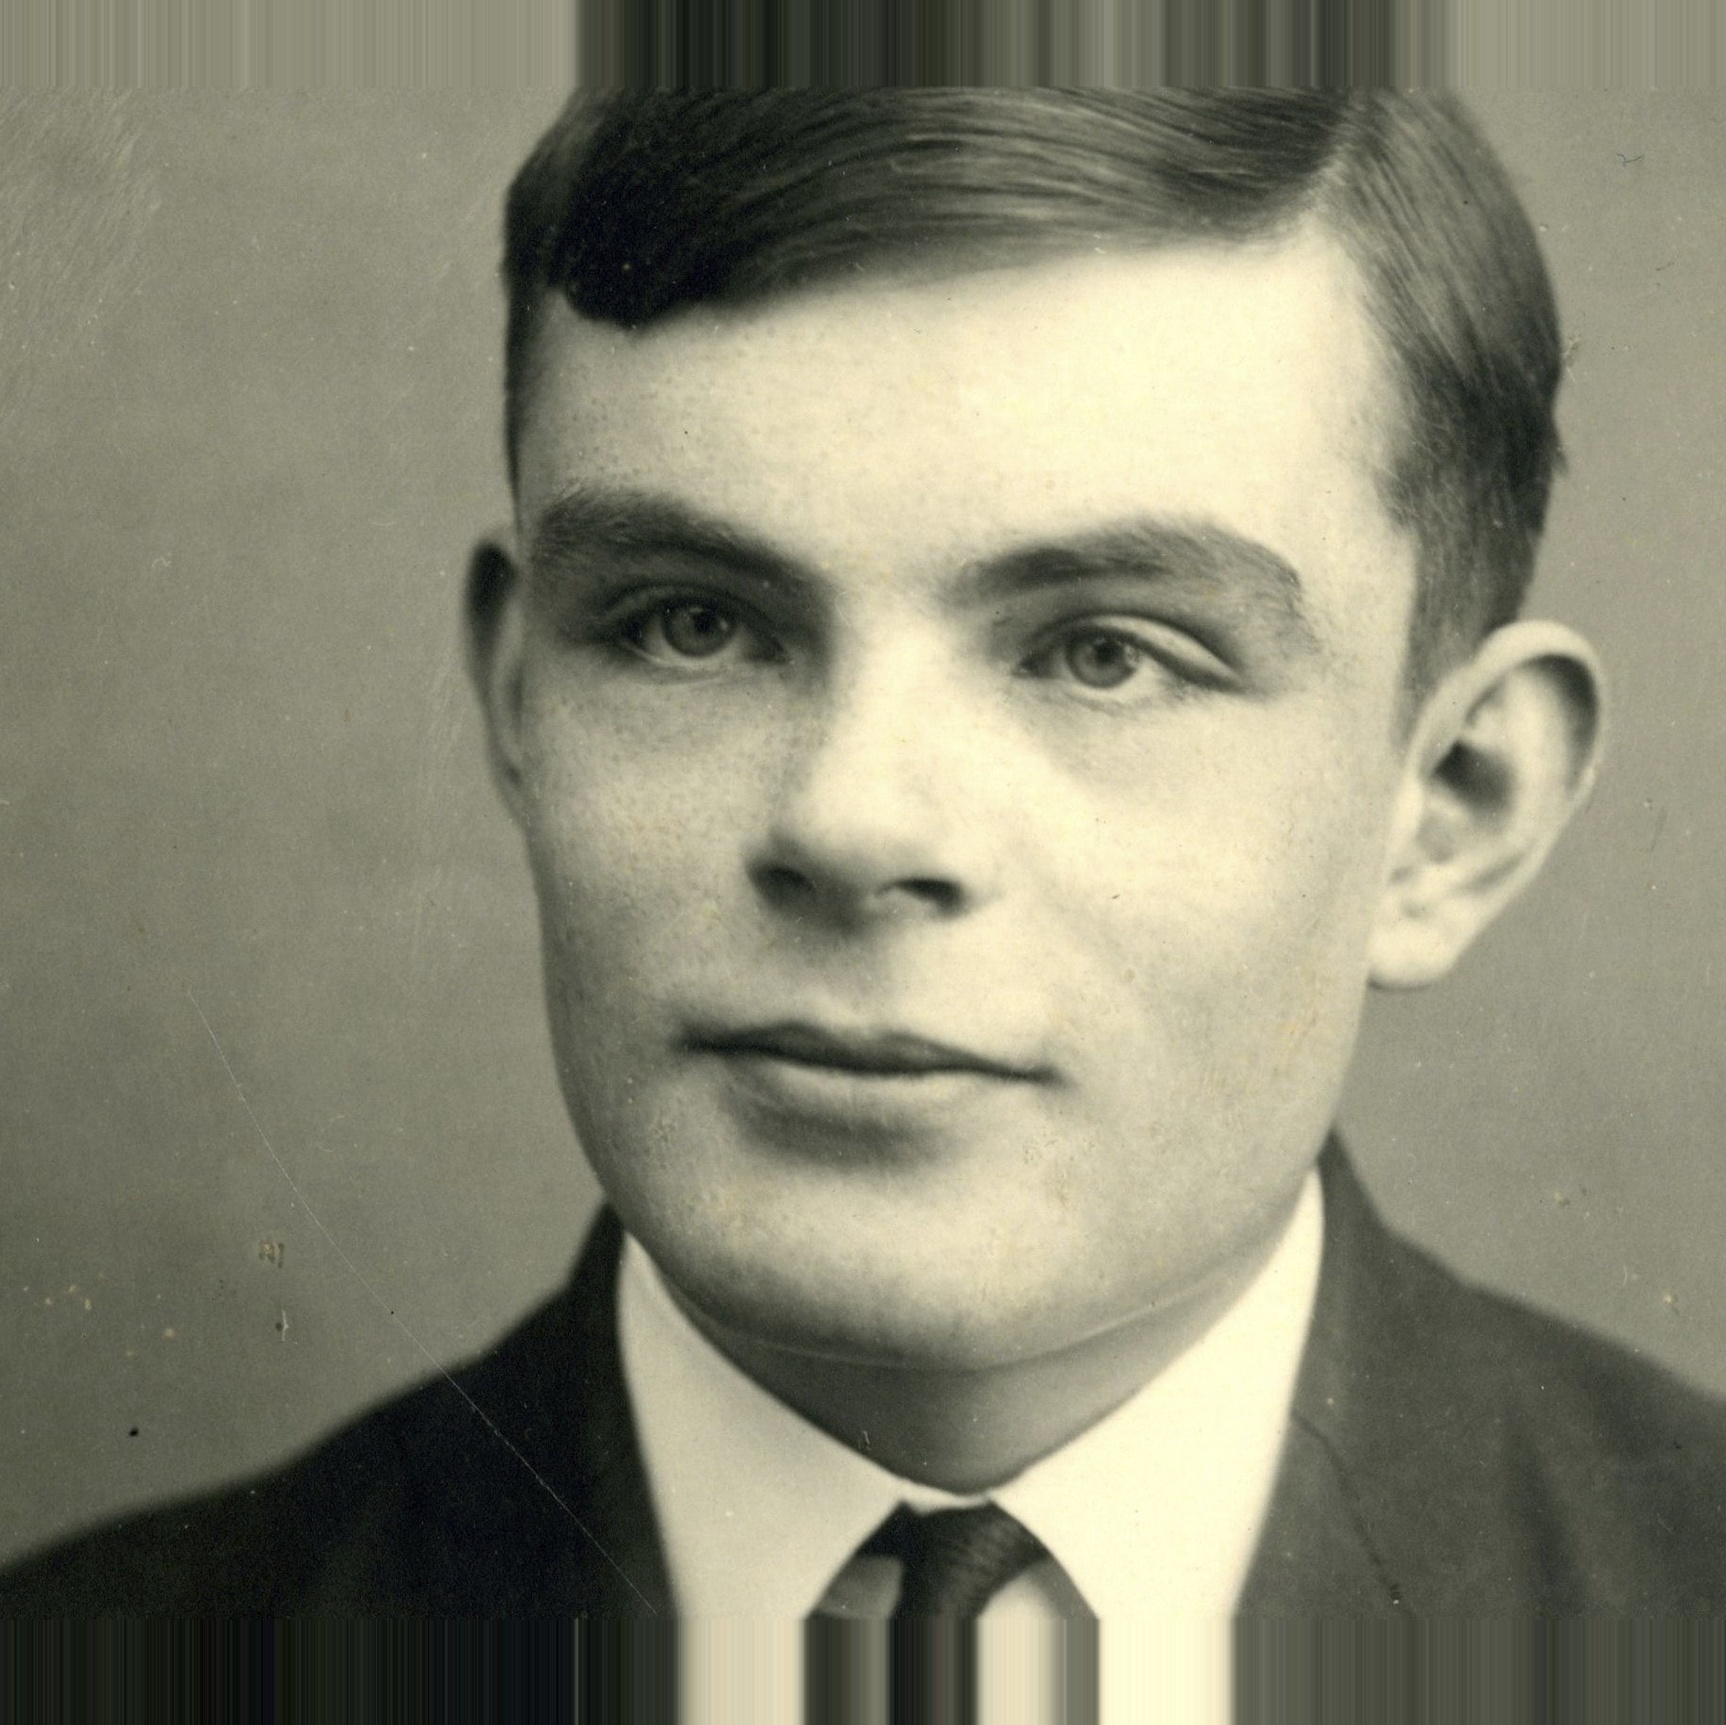
\includegraphics[height=5cm, width=\linewidth, keepaspectratio]{original_image_fgsm_1-eps1.jpg}
  \caption{Original sample classified as 28 years old}
\end{subfigure}
\begin{subfigure}{.5\textwidth}
  \centering
  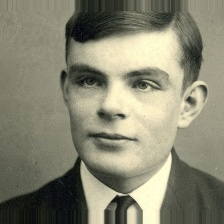
\includegraphics[height=5cm, width=\linewidth, keepaspectratio]{adversarial_image_fgsm_1-eps1.jpg}
  \caption{Adversarial sample classified as 59 years old}
\end{subfigure}

\begin{subfigure}{.5\textwidth}
  \centering
  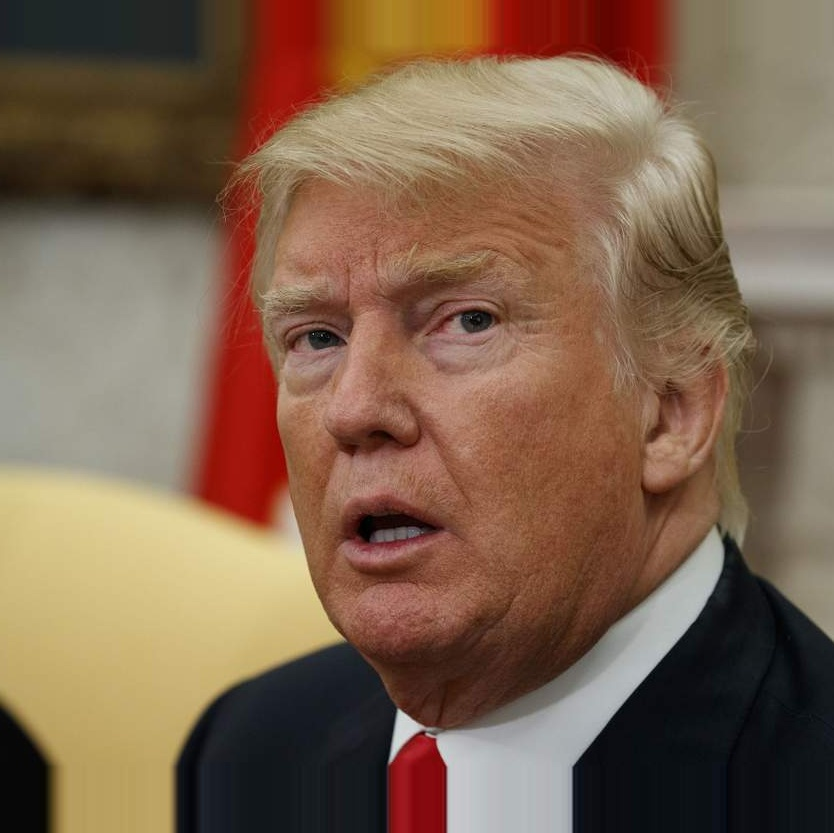
\includegraphics[height=5cm, width=\linewidth, keepaspectratio]{original_image_fgsm_2-eps1.jpg}
  \caption{Original sample classified as 59 years old}
\end{subfigure}
\begin{subfigure}{.5\textwidth}
  \centering
  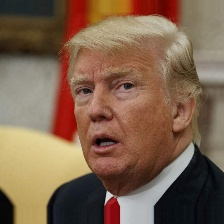
\includegraphics[height=5cm, width=\linewidth, keepaspectratio]{adversarial_image_fgsm_2-eps1.jpg}
  \caption{Adversarial sample classified as 28 years old}
\end{subfigure}

\begin{subfigure}{.5\textwidth}
  \centering
  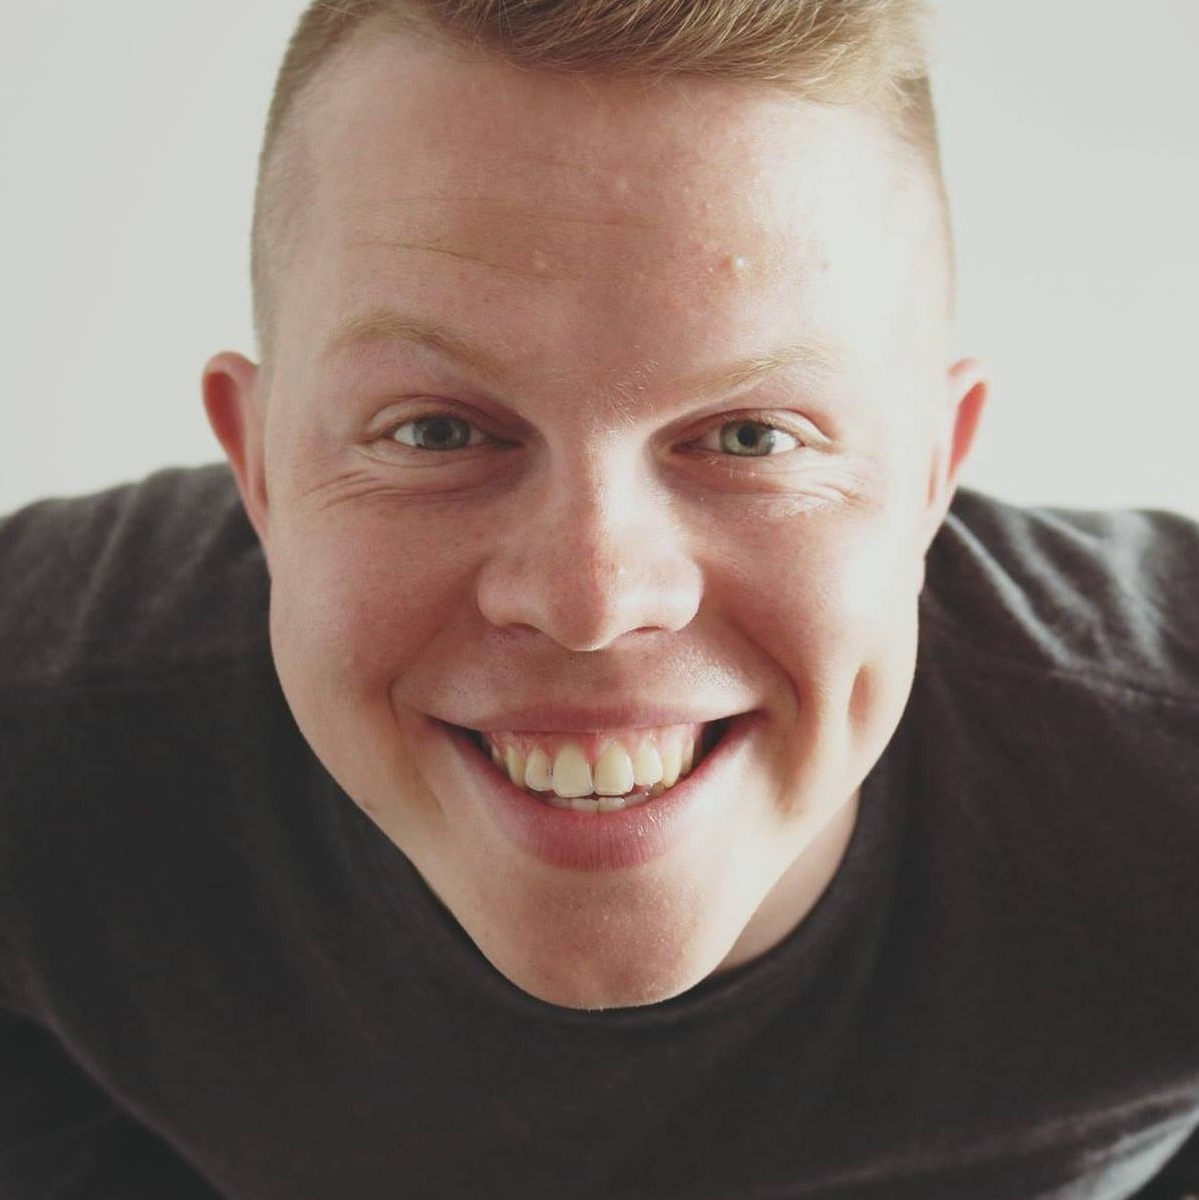
\includegraphics[height=5cm, width=\linewidth, keepaspectratio]{original_image_fgsm_3-eps1.jpg}
  \caption{Original sample classified as 28 years old}
\end{subfigure}
\begin{subfigure}{.5\textwidth}
  \centering
  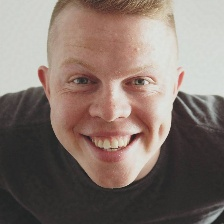
\includegraphics[height=5cm, width=\linewidth, keepaspectratio]{adversarial_image_fgsm_3-eps1.jpg}
  \caption{Adversarial sample classified as 64 years old}
\end{subfigure}

\caption{Original samples (left) and adversarial samples (right)}
\label{fig:motivational-samples}
\end{figure}

\section{Problem Definition} 
\label{motivation}
The assumption in the rest of this thesis is that the neural network is performing a \textit{classification task} - mapping an input (image) to a discrete output value (e.g. mapping an image of a traffic sign to the name of the traffic sign).  Output values are often called labels or categories. There is a finite number of possible labels.

To find errors in a system where a neural network is used, we need a framework which can trigger every possible output of the neural network.  We want to achieve that by using only one image as a starting point. 

Since for the same input we will always get the same output, modifications of that image are necessary. For each different desired output, a different modification of the image is performed.
Then we repeat that process by changing our desired output in every iteration and in that way, cover all possible outputs. The idea is that the modified image is as close as possible to the original one. For example, an image of a  \textit{STOP} sign can be modified as long as it still is an image of a  \textit{STOP} sign to a human observer. In that case, with the variations of the \textit{STOP} sign we cover all the possible outputs of the neural network - all other traffic signs. Using this technique, we can trigger errors in the system which can help us in the process of its verification. 

Modifying an input for a neural network with a goal of reaching an output that is different than the output of an unmodified input is an attack called \textit{misclassification}. If an output which an attacker wants to reach is one specific label, then a name of the attack is \textit{targeted misclassification}.

Creating a framework for targeted misclassification in the domain of age estimation as well as comparison and evaluation of existing approaches is the main focus of this thesis. In other words, the focus is on approaches how to trick a classifier to classify a person as older or younger than he or she actually is. 

\section{Aim of the Work}
To the best of my knowledge, nobody executed an attack against a DNN in the domain of age estimation yet. Hence, one of the first questions which this thesis aims to answer is the question whether already existing techniques can be used for attacks in this domain.

In order to further define aim of this work, an explanation of the major difference between two types of attacks against a neural network is necessary, namely the difference between \textit{white-box} attack and \textit{black-box} attack. 
In white-box attacks, an adversary has all the information about the DNN under attack. The internal structure of the neural network, all the implementation details and values of all the variables in any moment are known to the attacker. In other words, the attacker has access to the source code and nothing is hidden.
On the other hand, in black-box attacks an adversary doesn't have access to all the information. Depending on the precise definition of "black-box", more or less information is provided. In this thesis, the only capability of the black-box adversary is to observe the labels assigned by the DNN to chosen inputs.

A natural question is which algorithm is the best one for the white-box attack and which one for the black-box attack? Several algorithms are run in the different settings and results are compared. That provides an answer to the question which algorithm to use in which scenario.

Furthermore, in the domain of age estimation, it makes sense to be less strict about the targeted label. For instance, if an image of a minor is classified as an image of a person over a fifty years old, this could lead to the same consequences, no matter if it is classified as a 55 or 65 years old person. More precisely, if the goal is to hit any label from a specific group of labels, I define that attack as \textit{semi-targeted misclassification}. Of course, a group of labels must be smaller than a whole set of possible labels, otherwise the task is trivial. In general, this attack makes sense in any environment where labels can be clustered.

To this end, I adapted one already existing black-box approach is adapted to this more relaxed setting. Such a relaxation is not yet introduced in the literature since it is very domain specific. Consequently, the results can't be compared against previous work of that kind, but results are compared with targeted black-box misclassification attacks. This comparison is explained in more details in Section \ref{approach}. 

In terms of development, a DNN is implemented which receives an image as an input and outputs how old the person in the image is. In other words, a DNN for age estimation is trained. All the attacks are executed against this DNN. 

Next, the framework is constructed for a white-box and a black-box targeted misclassification attack. In other words, while treating the DNN as a white-box or a black-box, images  are constructed in a way that the targeted DNN outputs a specific year. Finally, the framework is extended with capability to craft semi-targeted black-box misclassification attacks.

\section{Methodological Approach} \label{approach}
The methodological approach consists of the following steps:
\begin{enumerate}
    \item I write about the background knowledge needed for training a neural network. The goal is to give a brief introduction to this area so that a non-expert reader can follow the rest of the thesis. Using that knowledge, I trained a deep neural network for age estimation of a person in the image.
    
    \item I conducted a research about different state of the art methods for generating \textit{adversarial examples}, i.e. images which are not correctly classified by DNN. The focus here is on the approaches that address targeted misclassification. While treating a DNN from the first step as a white-box, I use those methods to construct adversarial examples. Afterwards, I present and analyze the results of the attacks.
    
    \item I did a literature survey on the targeted black-box attack methods, explain those methods and use them to generate adversarial inputs for a DNN  from the first step, but this time while treating it as a black box. I compare the results of different algorithms.
    
    \item As the last step, combining the domain knowledge and an existing attack method, I implemented a new adversarial algorithm and using that algorithm, I construct images for semi-targeted misclassification. I compare results against targeted black-box approaches. The way I is compared them is the following: a target label for a targeted version of the attack is the median value of the set of labels in a semi-targeted version of the attack. If a DNN outputs any label outside the set of the labels, an attack is  considered as a successful no matter if it is a targeted or a semi-targeted misclassification attack.
\end{enumerate}


\section{Outline} 
In this chapter an introduction to the problem is provided. In the next chapter background knowledge is presented that is needed to follow the rest of the thesis. In Chapter \ref{chap:attacks} state-of-the-art attacks are presented and explained. In Chapter \ref{chap:experiments} results of the experiments are presented. The Semi-Targeted Approach is discussed in Chapter \ref{chap:semi-targeted}. Threats to validity and ideas for future work are presented in Chapter \ref{chap:threats}. Finally, summary of this thesis is presented in Chapter \ref{chap:summary}.



\chapter{Background}
A formal definition of a machine learning algorithm is given by \cite{Mitchell:1997:ML:541177}: "A computer program is said to learn from experience $E$ with respect to some class of tasks $T$ and performance measure $P$ if its performance at tasks in $T$, as measured by $P$, improves with experience $E$." 
From such a vague definition, it is obvious that a comprehensive introduction to machine learning is a broad topic. Hence, in this thesis a brief introduction to the \textit{image classification} problem is provided only. That should be enough for a non-expert to be able to read and to understand this whole thesis.

As explained in Section \ref{motivation}, an image classification is a task of assigning a \textit{label} or a \textit{class} to an image. If an input is $n$-dimensional vector and there are $k$ classes, then the learning algorithm is usually asked to produce a function $f: \mathbb{R}^n \rightarrow \{1, ... , k\}$. One other variant of a classification task would be to produce a function $f$ which outputs a probability distribution over classes, i.e. how likely each class is. In such a scenario, the next step usually is to assign a label according to the most likely class, but this must not be the case. A model that is used for classification task is called a \textit{classifier}.

After defining a task, it is important to know how to measure the performance of a model. Depending on the domain of a system, this measure can vary. The \textit{accuracy} of the model is usually measured for a classification task. It is the fraction of correct predictions of the model. For example, if the model was correct for 8 out of 10 samples, the accuracy of that model (on those 10 samples) is $0.8$ or $80\%$. An equivalent information can be obtained by measuring the \textit{error rate}. It is defined as the fraction of incorrect predictions of the model. 

Usually we are interested how good the model is on previously unseen data, because that way we can see how good will it work in the real world application. Therefore, we measure its performance on a set of data that is not used during training. Such a set of data is called \textit{test set}. A test set is subset of an entire \textit{dataset}.

A dataset is a collection of samples. One of the oldest datasets used in Machine Learning is the Iris flower dataset \cite{iris-dataset}. That dataset consists of 50 samples from each of three species of Iris. For each sample, four measures are taken: the length and the width of the sepals and petals, in centimeters. A measurable property of a sample is called a \textit{feature}. Hence, Iris dataset has 3 classes, 150 samples and each sample has 4 features. A classifier for that dataset could be modelled as a function $f: \mathbb{R}^4 \rightarrow \{0, 1, 2\}$ where $0, 1, 2$  encode the first, the second and the third type of Iris, respectfully.

Most machine learning algorithms have \textit{hyperparameters}, settings that we can use to control the algorithms' behaviour. Hyperparameters are values which are set before the learning algorithm begins. In contrast, the values of other parameters are derived via training. 

If a classifier has a high accuracy on a test dataset, we say it \textit{generalizes} well. However, if it has a high accuracy on the training samples, but a low accuracy on a test dataset, we say it \textit{overfits}. To avoid overfitting, training samples are split into two non overlapping subsets: the \textit{training} subset and the \textit{validation} subset.

The validation subset can be used to find good hyperparameters. The training subset is used to adjust parameters of a model. The validation subset is verifying that any increase in accuracy over the training dataset actually yields an increase in accuracy over a dataset that has not been shown to the model before, or at least the model hasn't been trained on it. If the accuracy over the training dataset increases, but the accuracy over the validation dataset stays the same or decreases, then a model is overfitting. The test accuracy, an accuracy we are typically interested in, is computed on the test dataset. That means that an original dataset is split into three disjoint subsets: training, validation and test subset. 

A problem can occur if there is not enough data, i.e. an original dataset is too small. That makes the training, the validation and the test subset not big enough. For instance, it can happen that the training dataset doesn't have any instance of some specific class or there is too few of them. That problem can be solved by the \textit{k-fold cross-validation} procedure.

That procedure is based on the idea of repeating the training and testing computation on different splits of the original dataset. The original set is split into $k$ equal disjoint subsets. Of the $k$ subsets, a single subset is retained as the validation set for testing the model, and the remaining $k-1$ subsets are used as training data. The process is then repeated $k$ times, with each of the $k$ subsets used exactly once as the validation data. The $k$ results can then be averaged to produce a test accuracy. 

So far, the basics of the machine learning are covered. A goal for the rest of this chapter is to provide a brief introduction to the deep learning area. In Section \ref{subsection:FNN} an introduction to the basic neural networks is provided. After that, in Section \ref{subsection:gradient-descent} the Gradient Descent algorithm and variations of it are introduced. Gradient descent is used for optimization of functions based on the derivations of them. The backpropagation algorithm, an efficient algorithm to compute a derivation of a function represented by a neural network, is introduced in Section \ref{subsection:backpropagation}. Finally, in Section \ref{subsection:convolutionalNN} convolutional neural networks are presented. A convolutional neural network represents a typical choice of the architecture of the neural network when it comes to the computer vision domain.

\section{Feedforward neural networks}
\label{subsection:FNN}
\textit{Feedforward neural networks} or \textit{multilayer peceptrons} (MLPs) are the essential deep learning models. A feedforward neural network defines a mapping $f (\pmb{x} ; \pmb{\theta}) = \pmb{y}$ and learns the value of the parameters $\pmb{\theta}$ that result in the best function approximation.

A neural network consists of several \textit{layers}. There is always one \textit{input} layer, followed by one or more \textit{hidden} layers and finally, there is an \textit{output layer}. The number of layers (without an input layer) defines a \textit{depth} of the model. There is no precise definition, but neural networks with more than three layers are called \textit{deep} neural networks. 

When it comes to feedforward neural networks, a network is a directed acyclic graph. Vertices of such a graph are called \textit{units} or \textit{neurons} and edges are called \textit{weights}. Vertices represent scalar functions of an input. Weights are the parameters $\pmb \theta$ which a neural network learns. Edges define data flow. One example of such a model is shown in the Figure \ref{fig:basic-cnn}.

\begin{figure}
\begin{tikzpicture}[
plain/.style={
  draw=none,
  fill=none,
  },
net/.style={
  matrix of nodes,
  nodes={
    draw,
    circle,
    inner sep=10pt
    },
  nodes in empty cells,
  column sep=2cm,
  row sep=-9pt
  },
>=latex
]
\matrix[net] (mat)
{
|[plain]| \parbox{1.3cm}{\centering Input\\layer} & |[plain]| \parbox{1.3cm}{\centering Hidden\\layer} & |[plain]| \parbox{1.3cm}{\centering Output\\layer} \\
& |[plain]| \\
|[plain]| & \\
& |[plain]| \\
  |[plain]| & |[plain]| \\
& & \\
  |[plain]| & |[plain]| \\
& |[plain]| \\
  |[plain]| & \\
& |[plain]| \\    };
\foreach \ai [count=\mi ]in {2,4,...,10}
  \draw[<-] (mat-\ai-1) -- node[above] {Input \mi} +(-2cm,0);
\foreach \ai in {2,4,...,10}
{\foreach \aii in {3,6,9}
  \draw[->] (mat-\ai-1) -- (mat-\aii-2);
}
\foreach \ai in {3,6,9}
  \draw[->] (mat-\ai-2) -- (mat-6-3);
\draw[->] (mat-6-3) -- node[above] {Ouput} +(2cm,0);
\end{tikzpicture}

\caption{An example of the feedforward neural network architecture}
\label{fig:basic-cnn}
\end{figure}

A typical architecture of one neuron can be seen in the Figure \ref{fig:basic-neuron}. That specific neuron performs an operation $ f(net) = y $ where $net = x1*w1 + x2*w2 + x3*w3 + bias$.  Bias is usually modelled as an additional input with the corresponding weight $w=1$. Then a neuron performs the operation $ f(\pmb x \times \pmb w) = y$ where $\times$ denotes cross-product between two vectors. Function $f$ is called an \textit{activation function} and usually is the same for all neurons in the same layer. In the input layer the activation function is mapping from input to output, i.e. $f(x) = x$, but in the other layers those are usually non-linear functions. 

 \textit{Convolutional Neural Networks} (CNNs), which are described in Subsection \ref{subsection:convolutionalNN}, are a specific kind of feedforward neural networks. They are most popular in the computer vision domain. If there are cycles in a graph, we are probably talking about the \textit{Recurrent Neural Networks} (RNNs) which are used in domains where a context is important, for instance in Natural Language Processing. However, RNNs are out of the scope of this thesis and will not be further discussed.

\begin{figure}
\begin{tikzpicture}[
init/.style={
  draw,
  circle,
  inner sep=2pt,
  font=\Huge,
  join = by -latex
},
squa/.style={
  draw,
  inner sep=2pt,
  font=\Large,
  join = by -latex
},
start chain=2,node distance=13mm
]
\node[on chain=2] 
  (x2) {$x_2$};
\node[on chain=2,join=by o-latex] 
  {$w_2$};
\node[on chain=2,init] (sigma) 
  {$\displaystyle\Sigma$};
\node[on chain=2,squa,label=above:{\parbox{2cm}{\centering Activation \\ function}}]   
  {$f$};
\node[on chain=2,label=above:Output,join=by -latex] 
  {$y$};
\begin{scope}[start chain=1]
\node[on chain=1] at (0,1.5cm) 
  (x1) {$x_1$};
\node[on chain=1,join=by o-latex] 
  (w1) {$w_1$};
\end{scope}
\begin{scope}[start chain=3]
\node[on chain=3] at (0,-1.5cm) 
  (x3) {$x_3$};
\node[on chain=3,label=below:Weights,join=by o-latex] 
  (w3) {$w_3$};
\end{scope}
\node[label=above:\parbox{2cm}{\centering Bias \\ $b$}] at (sigma|-w1) (b) {};

\draw[-latex] (w1) -- (sigma);
\draw[-latex] (w3) -- (sigma);
\draw[o-latex] (b) -- (sigma);

\draw[decorate,decoration={brace,mirror}] (x1.north west) -- node[left=10pt] {Inputs} (x3.south west);
\end{tikzpicture}
\caption{A single processing unit in a neural network}
\label{fig:basic-neuron}
\end{figure}

\section{Gradient descent}
\label{subsection:gradient-descent}
The accuracy of a parametric model depends on the data provided to train it and the parameters used. The same holds for neural networks. The parameters in the neural networks are weights and during the training we are trying to find \textit{the best} weights. To find them, we express how bad the model is using the \textit{loss function} or \textit{cost function}. It expresses how wrong the model is (for a given data) using the given weights. When such a function is defined, all we do is try to find an input to that function, i.e. weights, such that output of that function, i.e. loss, is minimal. Most machine learning algorithms have some kind of optimization built in. Optimization refers to the task of find $\pmb x$ s.t. $f(\pmb x)$ is maximal or minimal. In this thesis, optimization will always mean minimization, except when stated otherwise. Maximization can be accomplished by minimizing the function $-f(\pmb x)$.

Since training a neural network is actually minimizing a loss function that is represented by the neural network, two things need to be decided: the loss function that will be used and the optimization algorithm that will be used to find its minimum.

The most popular classification loss function is \textit{cross-entropy}. Given two probability mass functions (a mass function is a function that gives the probability that a discrete random variable is exactly equal to some value) $\pmb u$ and $\pmb v$ in $\mathbb{R}^T$, i.e. $\pmb u = (u_1, ..., u_T)$ and $\pmb v =  (v_1, ..., v_T)$, the cross-entropy between $\pmb u$ and $\pmb v$ is
 \begin{equation}
H (\pmb u, \pmb v)= - \sum_{t=1}^T  u_t  \text{ln} v_t 
\end{equation}

Let $\pmb u$ enocde the ground-truth label, $u_c = 1$ where $c$ is index of the class. Let $\pmb v$ be the predicted softmax class scores. Now $H$ measures how dissimilar true and predicted probabilities are for a single sample.

Let $\mathcal{D}$ be a dataset such that
$ \mathcal{D} = \{ (\pmb x_s, \pmb w_s)\}_{s=1}^{S}$ where $x_s$ is an input vector and $w_s$ is a vector encoding the ground truth (i.e. all indices have value $0$, except on the index of the class which $x_s$ represents where the value is $1$).

On this basis, \textit{cross-entropy loss} on $\mathcal{D}$ is defined as
\begin{equation} \label{eq:loss-function}
L(\pmb \theta) = \frac{1}{S} \sum_{s=1}^{S} H (\pmb w_s, \text{softmax} (f(\pmb x_s ; \pmb \theta)))
\end{equation}

Models trained with this loss function are called \textit{softmax classifiers}. If $T = 2$, it is also called \textit{logistic regression}. Classifiers learn to predict probabilities per class label.

After we defined the loss function $L(\pmb \theta)$  as in \ref{eq:loss-function}, we need to find an optimization algorithm to find its minimum. Since the function is not linear in $\pmb \theta$, a nonlinear optimization algorithm is needed. A popular choice in deep learning is \textit{Gradient Descent}.

Gradient Descent is an iterative optimization algorithm that is used for finding the minimum of a function. It is based on the first derivative of the function whose minimum needs to be found. This means that the function must be differentiable. 

Let $\nabla f$ be a vector of all partial derivatives of a function $f: \mathbb{R}^N \mapsto \mathbb{R}^N$. Then $\nabla f(\pmb x) = (f_{x_1}(\pmb x), ..., f_{x_n}(\pmb x))$  encodes how fast $f$ changes with all arguments $x_1, ..., x_n$, which is exactly what is needed for optimizing $L(\pmb \theta)$. Compute the direction of the greatest increase, i.e. $\nabla L(\pmb \theta)$, and move in the opposite direction. The size of that move is called \textit{step size} and it is defined by the \textit{learning rate} - hyperparameter $\alpha$.  

The pseudo code for gradient descent is presented in Algorithm \ref{alg:gradient-descent}.

\begin{algorithm}[htb]
\caption{Gradient Descent}
\label{alg:gradient-descent}

\KwIn{$\pmb \theta, L, \alpha $}

\While {$true$}{
    $\pmb \theta^{'} \leftarrow \nabla L(\pmb \theta)$\;
    \If {$\| \pmb \theta^{'}\|  \approx 0 $} {
    		\Return\;
    }
    $\pmb \theta \leftarrow \pmb \theta - \alpha * \pmb \theta^{'}$\;
}
\end{algorithm}

This algorithm is simple and efficient. Simple since the only requirement is that $f$ is differentiable and efficient because it requires only first derivatives. A problem that can occur is that $\| \pmb \theta^{'}\|  \approx 0$ can happen at all critical points - minimum, maximum and saddle points.

To speed up convergence, \textit{momentum} is introduced using hyperparameter $\beta$. It increases step size dynamically by using $velocity$ $\pmb v$. Velocity builds up momentum if successive gradients are similar. The pseudo code for gradient descent with momentum is shown in Algorithm \ref{alg:gradient-descent-momentum}

\begin{algorithm}[htb]
\caption{Gradient Descent with momentum}
\label{alg:gradient-descent-momentum}

\KwIn{$\pmb \theta, L, \alpha, \beta $}

$\pmb v \leftarrow \pmb 0$\;
\While {$true$}{
    $\pmb \theta^{'} \leftarrow \nabla L(\pmb \theta)$\;
    \If {$\| \pmb \theta^{'}\|  \approx 0 $} {
    		\Return\;
    }
    $\pmb v \leftarrow  \beta \pmb v - \alpha * \pmb \theta^{'}$\;
    $\pmb \theta \leftarrow \pmb \theta + \pmb v$\;
}
\end{algorithm}

The idea behind gradient descent with \textit{Nesterov Momentum}, which works often better than standard Gradient Descent with momentum, is not to evaluate the gradient at the current point, but at the point which would be the next, i.e. evaluate the gradient at $\pmb \theta + \pmb v$ instead of at $\pmb \theta$. The pseudo code is shown in Algorithm \ref{alg:gradient-descent-nesterov-momentum}

\begin{algorithm}[htb]
\caption{Gradient Descent with Nesterov momentum}
\label{alg:gradient-descent-nesterov-momentum}

\KwIn{$\pmb \theta, L, \alpha, \beta $}

$\pmb v \leftarrow \pmb 0$ \;
\While {$true$}{
    $\pmb \theta^{'} \leftarrow \nabla L(\pmb \theta + \pmb v)$\;
    \If {$\| \pmb \theta^{'}\|  \approx 0 $} {
    		\Return\;
    }
    $\pmb v \leftarrow  \beta \pmb v - \alpha * \pmb \theta^{'}$\;
    $\pmb \theta \leftarrow \pmb \theta + \pmb v$\;
}
\end{algorithm}

So far, $L(\pmb \theta)$ is computed based on the whole training dataset $\mathcal{D}$. Therefore, time complexity increases linearly with number of samples in $\mathcal{D}$. That can be problematic if $\mathcal{D}$ is large. Instead of having a whole dataset $\mathcal{D}$ as a \textit{batch}, we can evaluate $L(\pmb \theta)$ on a subset of the training dataset with $S$ number of samples. If $S = |\mathcal{D}|$, it is called \textit{Batch Gradient descent}. But we can split the training dataset $\mathcal{D}$ into several \textit{minibatches} (subsets) of cardinality $S$ and process them one by one (one per iteration). One full run through the training set is called an \textit{epoch}. Usually training takes many epochs. The resulting algorithm is called \textit{Minibatch Gradient Descent} (or \textit{Stochastic Gradient Descent} (SGD) if $S = 1$). In practice, it is often called SGD even if $S > 1$. The time for a single iteration is now independent of the dataset size and depends only on the size of a minibatch. Typically, $S$ is 64, 128, 256 or 512. In general, $S$ is usually $2^{N}$ because of efficiency reasons (data parallelism). Decreasing $S$ decreases the computation time per iteration, the amount of memory required on GPU (minibatch processed as whole) and the accuracy of the gradient estimate. It is important to sample minibatches randomly to break (possible) ordering in a dataset. In practice, usually training set is shuffled once or before every epoch and then processed sequentially in minibatches. 


There are many alternatives to the gradient descent algorithm which have an advantage of not having to choose the learning rate. An interested reader can find an overview of gradient descent optimization algorithms in \cite{gradient-descent-overview}. 





\section{Backpropagation}
\label{subsection:backpropagation}
Now we already know how to train a neural network. We can use a cross-entropy loss function $L (\pmb \theta)$ and minibatch gradient descent with (Nesterov) momentum. For gradient descent, we must calculate $\nabla L (\pmb \theta)$.

One way to obtain $\nabla L (\pmb \theta)$ is \textit{numerical differentiation}. 
Let $p \in [1, dim(\pmb \theta)]$, $\epsilon \in \mathbb{R}$ be arbitrary small, and $\pmb 1_p$ be a vector which is $1$ at position $p$ and $0$ otherwise. Then directly by definition of the derivative we obtain \ref{eq:numerical-derivative-1}

\begin{equation}\label{eq:numerical-derivative-1}
\nabla L (\pmb \theta) = (L(\pmb \theta + \pmb 1_p \epsilon) - L (\pmb \theta)) / \epsilon
\end{equation}

Sometimes is \ref{eq:numerical-derivative-2} used instead of \ref{eq:numerical-derivative-1}.
\begin{equation}\label{eq:numerical-derivative-2}
\nabla L (\pmb \theta) = (L(\pmb \theta + \pmb 1_p \epsilon) - L (\pmb \theta - \pmb 1_p \epsilon)) / 2 \epsilon
\end{equation}

This approach is easy to implement, but it's only an approximation ($\epsilon$ cannot be arbitrary small) and it is too inefficient in practice because $L$ must be evaluated $dim(\pmb\theta)$ times (modern DNNs have millions of parameters). Instead of \textit{numerical differentiation}, preferable way is to obtain $\textit{analytic gradient}$, i.e. obtain $\nabla L (\pmb \theta)$ analytically using calculus. This approach is more accurate (no approximation) and much more efficient (single evaluation).


A neural network is actually a computational graph composed of other functions. The loss function $L$ of the neural network is again a computational graph. Derivatives in such graphs can be computed iteratively using the \textit{chain rule}. The chain rule is used for computing the derivative of composition of two or more functions. 

Let $f: \mathbb{R} \mapsto \mathbb{R}$, $g: \mathbb{R} \mapsto \mathbb{R}$ and $F: \mathbb{R} \mapsto \mathbb{R}$ s.t. $F(x) = f(g(x))$. Then by the chain rule, $F'(x) = f'(g(x))g'(x)$.

Based on the chain rule, the gradient of every weight can be efficiently computed and then updated as defined in the gradient descent method. The paper in which this famous algorithm is introduced is \cite{Rumelhart:1986:LIR:104279.104293}.

\section{Convolutional neural networks}
\label{subsection:convolutionalNN}
Since the focus of this thesis is on the computer vision domain, this background chapter wouldn't be complete without mentioning the most popular choice of neural networks for image classification, namely \textit{Convolutional Neural Networks} (CNNs/ConvNets).

Convolutional Neural Network is a well-known deep learning architecture inspired by the natural visual perception mechanism of living creatures. Among different types of deep neural networks, CNNs have been most extensively studied. ConvNets are feed-forward neural networks which contain one or more \textit{convolutional layers}. Neurons in this architecture are purposely spatially arranged to form feature maps. ConvNet architectures make the explicit assumption that the inputs are images, which allows a creator of it to encode certain properties into the architecture. These properties make the forward function more efficient to implement and vastly reduce the amount of parameters in the network.

Unlike a regular Neural Network as introduced in the previous subsection, the layers of a ConvNet have neurons arranged in 3 dimensions: width, height, depth (not the same as depth of the network). This makes sense, because an image has width, height and number of channels (depth). To reduce number of parameters, the neurons in a layer are only connected to a small fixed-size region of the layer before it and weights are shared among neurons in the same feature map (layer). Such a layer is called a convolutional layer. Except for convolutional layers, in the CNN architecture, there are usually \textit{Pooling Layers} (POOL) and \textit{Fully-Connected Layers} (FC), which are classic layers as introduced in a previous subsection. In CNNs, activation functions are also often referred to as separate layers. One of the most popular activation functions among CNNs is the \textit{ReLU} activation function. It is defined as in  \ref{eq:relu}
\begin{equation}\label{eq:relu}
f(x) = max (0, x)
\end{equation}
and its graph can be seen in the Figure \ref{fig:relu}.

\begin{figure}[!ht]
\centering
\begin{tikzpicture}
\begin{axis}[
xlabel={$x$},
ylabel={$f(x)$},
clip=false,
grid=major,
xmin=-6, xmax=6,
ymin=-1, ymax=6,
domain=-6:6
]
 \addplot+[mark=none,smooth, blue,domain=-6:0] {0};
  \addplot+[mark=none,smooth, blue,domain=0:6] {x};
\end{axis}
\end{tikzpicture}
\caption{ReLU function}
\label{fig:relu}
\end{figure}

Pooling Layers are used to perform a downsampling operation along the spatial dimensions (width, height). After all, we must reduce an input image dimensions to produce an output of expected dimensions.  It is common to periodically insert a Pooling layer in-between successive convolutional layers in a ConvNet architecture.

A simple CNN for classification could have the architecture [INPUT - CONV - RELU - POOL - FC]. A similar architecture is shown in the Figure \ref{fig:cnn}.

 For more information about CNNs, please consider the original paper\cite{krizhevsky2012imagenet}. 
 
\begin{figure}[h]
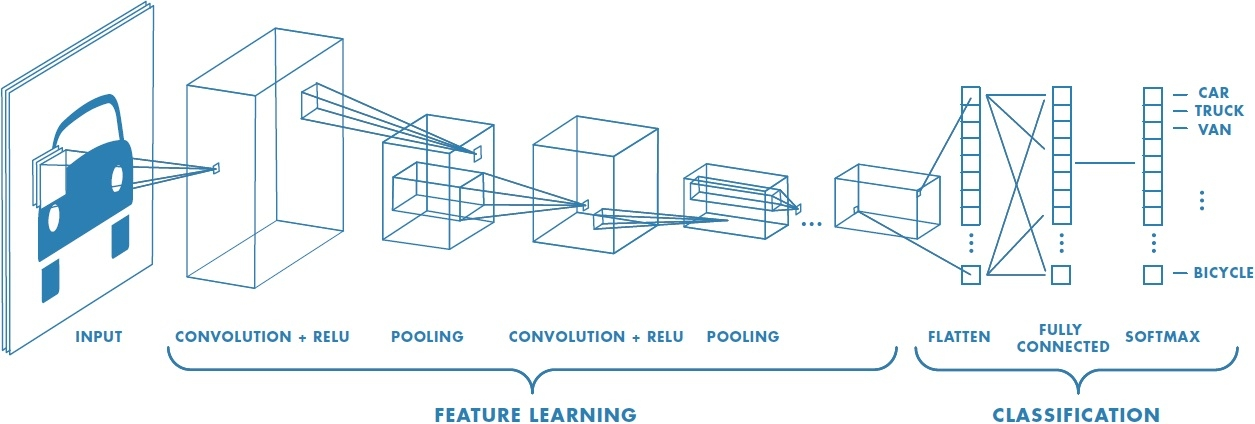
\includegraphics[width=13cm]{cnn}
\caption{A simple deep neural network, image taken from \url{floydhub.com}}
\label{fig:cnn}
\end{figure}



\chapter{State-of-the-Art}
\label{chap:attacks}
Machine learning (ML) is a rapidly evolving field and a lot of papers have been published in ML area in the last few years. However, since the focus of this master thesis is on generating adversarial examples, the related work can be separated into two categories, one in which DNNs are treated as a white-box and one where they are treated as a black-box. 

In terms of white-box attacks, the \textit{Fast Gradient Sign Method} (FGSM) attack is presented  in \cite{fgsm-original}. The attack computes an adversarial image for a non-targeted attack based on the direction of the gradient of a DNN. The FGSM attack is presented in more details in Section \ref{sec:FGSM}.

In \cite{DBLP:journals/corr/PapernotMJFCS15}, the \textit{Jacobian-based Saliency Map Attack} (JSMA) for generating adversarial examples is introduced. The attack is based on identifying regions in an image which have a higher impact on a DNN's output during the classification. JSMA attack is presented in more details in  Section \ref{sec:JSMA}.

In \cite{DBLP:journals/corr/CarliniW16a}, the \textit{Carlini \& Wagner} (CW) attack is presented. The attack is based on formulating an attack as an optimization problem and then using a state-of-the-art optimizer to solve it. The attack is presented in more details in Section \ref{sec:CW}.

All three attacks, FGSM, JSMA, and CW are evaluated in the experiments in this thesis.

On the black-box side of the attacks, the \textit{transfer-based} approach introduced in \cite{DBLP:journals/corr/PapernotMGJCS16} is a popular choice. This approach uses a subsitute DNN that is trained on a similar dataset as the targeted DNN. More details about the transfer-based approach can be found in Section \ref{sec:transfer-based}.

In \cite{ensemble-attack}, the authors show that adversarial samples for a targeted misclassification don't transfer as well as in a pure misclassification attack. The authors suggest an \textit{ensemble} approach which is described in Section \ref{sec:ensemble-approach}.

In \cite{brendel2018decisionbased}, the authors implement a completely different attack and call it \textit{Boundary Attack}. The attack starts with an image of a targeted class and then, step by step, the image is changed to an image of some other class while staying adversarial, i.e. classified as a target class by a DNN under the attack. The boundary attack is described in Section \ref{sec:boundary-attack}.

I direct the interested reader to the survey \cite{survey} of the different attack strategies and defenses for a more detailed overview.

\section{Fast Gradient Sign Method (FGSM)}
\label{sec:FGSM}
Let $\pmb \theta$ be the parameters of a model, $\pmb x$ the input to the model, $y$ the target associated with $\pmb x$, and $J (\pmb \theta, \pmb x, y)$ be the cost fucntion used to train the neural network. Then an adversarial perturbation is computed as 
\[ 
\pmb \rho = \epsilon * sign (\nabla_{\pmb x} J(\pmb \theta, \pmb x, y)).
\]

An adversarial example can be crafted then by adding the adversarial perturbation to the original input

\[\pmb x = \pmb x + \pmb \rho .\]
 
 
The FGSM attack perturbs an image to increase the loss of the classifier on the resulting image. The target label in the original paper \cite{fgsm-original} was always a label with the least probability for an unmodified image. The authors evaluate their method on the ImageNet dataset \cite{datasetImageNet}, a dataset used for a large-image recognition task with 1000 classes, and achieve good results for misclassification. Targeted misclassification was not evaluated. Similar results are achieved on the MNIST dataset 	\cite{datasetMNIST}, a dataset used for a digit-recognition task (0-9), and on the CIFAR-10 dataset \cite{datasetCIFAR10}, a dataset used for a small-image recognition task, also with 10 classes as in MNIST. From Figure \ref{fig:gibbon}, a reader can get the intuition for the attack. For more details, please consult the original paper.

\begin{figure}[h]
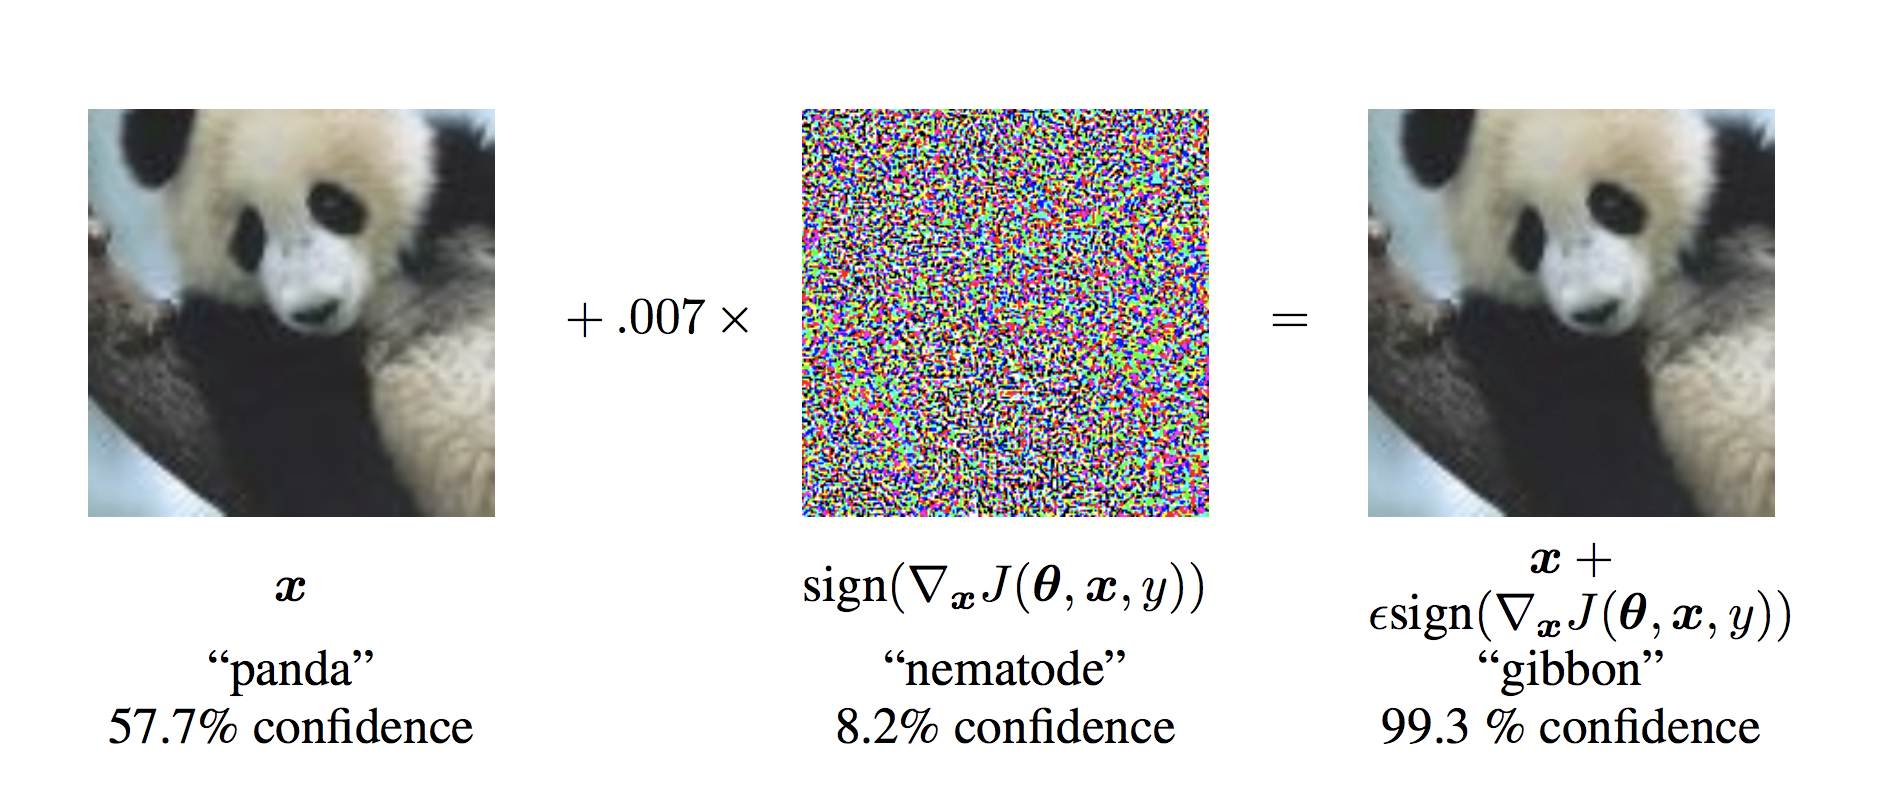
\includegraphics[width=13cm]{gibbon}
\caption{Image taken from the \cite{fgsm-original}}
\label{fig:gibbon}
\end{figure}




\section{Jacobian-based Saliency Map Attack (JSMA)}
\label{sec:JSMA}
This attack is based on a greedy algorithm that picks pixels to modify one at a time, increasing the the likelihood of the targeted class in each iteration.  \textit{Adversarial Saliency Maps} - maps that measure an impact of a pixel on an image being classified as a target class - are created. If a value in this map is large, it means that changing that pixel will increase the likelihood of the image being classified as a target class. 

The idea is, given the saliency map for a target class, the algorithm picks the pixel with the highest impact and modifies it. In the next iteration, the second most important pixel is changed and so on. This continues until either the attack succeeds to trick the classifier or too many pixels get changed and the attack becomes detectable. In the actual implementation of the algorithm, instead of picking one pixel, a pair of pixels is picked.

Formally, let $t$ be the target class, $\pmb x$ be the input to the classifier and $\pmb F$ be the output of the softmax layer. Then the adversarial saliency map in terms of pair pixels $p, q$ is defined as:

\[
\alpha_{pq} = \sum_{i \in \{p,q\}} \frac{\partial \pmb F(\pmb x)_t}{\partial \pmb x_i},
\]

\[
\beta_{pq} = ( \sum_{i \in \{p,q\}} \sum_{j \neq t} \frac{\partial \pmb F (\pmb x)_j }{\partial \pmb x _i}) - \alpha_{pq}
\]

so that $\alpha_{pq}$ represents the impact of changing the both pixels $p$ and $q$ on the input being classified as $t$, and $\beta_{pq}$ represents how
much changing $p$ and $q$ will change all the other outputs of the softmax layer.

Now the algorithm picks $p$ and $q$ such that the target class gets more likely ($\alpha_{pq} > 0$), but other classes get less likely ($\beta_{pq} < 0$) and that combination is as strong as possible, i.e. that $ - \alpha_{pq} * \beta_{pq}$ is as large as possible. This can be formalized as:

\begin{align*}
(p^*, q^*) 
				&= arg max_{p, q} (- \alpha_{pq} * \beta_{pq}) \\
                  & \textnormal{ s.t. } \alpha_{pq} > 0 \textnormal{ and } \beta_{pq} < 0
\end{align*}


Starting with an original input, two by two pixels are picked and perturbed by a constant offset $\epsilon$. The authors \cite{DBLP:journals/corr/PapernotMJFCS15} show that JSMA attack can effectively produce MNIST samples that are correctly classified by human subjects, but misclassified into a specific target class by a DNN with a high success rate. 

 
\section{Carlini \& Wagner (CW)}
\label{sec:CW}
% L norm introduction

To quantify similarity between two images, different distance metrics can be used. Quantification of similarity can be used when comparing how much an adversarial image is different from the original input. There are three widely-used distance metrics in the literature for generating adversarial examples , all of which are $L_p$ distances. The $L_p$ distance is written $||x - x'||_p$, where the $p$-norm is can be defined as

\begin{equation}
  ||v||_p=\left\{
  \begin{array}{@{}ll@{}}
       |\{i | v_i \neq 0 \}|, & \text{if } p = 0 \\
    ( \sum_{i = 1}^{n} |v_i|^p)^{1/p}, & \text{if } p \in [1, \infty) \\
    max\{|v_1|, |v_2|, ..., |v_n|\} & \text{if } p = \infty
  \end{array}\right.
\end{equation} 

In other words, $L_0$ measures how many pixels are changed, $L_2$ measures standard euclidean distance and $L_\infty$ measures the maximum change to any of the coordinates. It is open for discussion which metric performs the best job in measuring the human perceptual of similarity, but neither of the $L_p$ metrics is optimal for that.

% end of L norm introduction

The authors \cite{DBLP:journals/corr/CarliniW16a} introduce three new attacks for the $L_0$, $L_2$, and $L_{ \infty }$ distance metrics. It is worth mentioning that their $L_0$ attack is the first published attack which can cause targeted misclassification on the ImageNet dataset. All three of them are based on optimization techniques.

In this thesis, $L_2$ is used in the attack and hence I explain it now.

Let $t$ be the target class, $\pmb Z$ be the output of the targeted DNN before the softmax layer with $\pmb Z_i$ as an output for the class $i$, $\kappa$ a parameter that controls the confidence with which the misclassification occurs, $c$ a constant value, and $\pmb x$ be the original input.
Given $\pmb x$ and the target class $t$, search for $\omega$ that solves

\[
argmin_{\omega} ||\frac{1}{2}*(tanh(\omega) + 1) - \pmb x||_2^2 + c * f(\frac{1}{2}(tanh(\omega) + 1))
\]
with $f$ defined as 
\[
f(\pmb x') = max(max\{\pmb Z(\pmb x ')_i : i \neq t\} - \pmb Z(x)_t, - \kappa).
\]

The unrestricted perturbation $\pmb \delta^*$ is then defined as 
\[
	\pmb \delta^*_i = \frac{1}{2} * (tanh ( \omega_i) + 1) - \pmb x_i
\]
and after converting it to the restricted perturbation $\pmb \delta$ (details in the original paper \cite{DBLP:journals/corr/CarliniW16a}), an adversarial example $\pmb x^*$ is produced as 
\[
\pmb x^* = \pmb x +\pmb  \delta.
\]

According to the authors, this attack is often much more effective (and never worse) than all the others presented in the literature. Attacks are evaluated on the three datasets: ImageNet, MNIST and CIFAR-10. They also report that the JSMA attack, an attack introduced in Section \ref{sec:JSMA}, is always failing on the ImageNet dataset due to memory complexity of the algorithm, i.e. dimensions of images in ImageNet dataset are too big for JSMA attack. This implies that the JSMA attack would not work in my thesis as well if an image of a person is too big. Reported results for the CW attack are showing 100\% success against all three datasets.










\section{Transfer based approach}
\label{sec:transfer-based}
This technique is used to attack the DNN in the black-box settings. The idea is to create a \textit{substitute} DNN which should be similar to the targeted DNN. A precise definition of the similarity is omitted here because it's not well defined, but the substitute DNN should solve the same task as the targeted DNN.

Adversarial images are crafted then for a substitute DNN using a white-box approach, for instance the FGSM attack introduced in Section \ref{sec:FGSM}. Created adversarial images are used then as adversarial images for the black-box DNN as well. The main idea is that similar classifiers will have similar boundaries for a specific class and therefore the same adversarial example should be adversarial for both networks. 

The dataset on which the substitute neural network is trained should be similar to the dataset on which the targeted neural network is trained. Ideally, that would be the same dataset, but the assumption is that an attacker doesn't have access to that data. 

The attacker therefore generates a Synthetic Dataset. He or she starts generating the dataset by querying the targeted DNN with several examples and obtaining labels for them. Afterwards, he or she expands the dataset using the Jacobian-based Dataset Augmentation and trains the substitute neural network. For more details how to generate the synthetic dataset, please consult the original paper  \cite{DBLP:journals/corr/PapernotMGJCS16}.

The Authors present good results for misclassification attacks against the MNIST dataset and the GTSRD dataset \cite{datasetGTSRD}. Targeted misclassification is not presented in the paper.


\section{Ensemble approach} 
\label{sec:ensemble-approach}
This approach is also based on transferability of an adversarial image, but instead of generating an adversarial image for one neural network, generates it for several of them. The underlying assumption is that if an adversarial example works as expected among several models, it will work as expected for the one more as well. Both approaches will be implemented - when a substitute network is only a single neural network, and when there is several of them. I want to see if it's enough to use only one neural network as a substitute to achieve good results in semi-targeted misclassification.



\section{Boundary attack}
\label{sec:boundary-attack}
This approach is also used in black-box settings and it is completely different than attacks introduced in Sections \ref{sec:transfer-based} and \ref{sec:ensemble-approach}. Boundary attack has nothing to do with neither a substitute DNN nor transferability of the adversarial examples. 

The attack starts with an image of a targeted class and then, step by step, it changes it to an image of some other class while staying adversarial, i.e. classified as a target class by a DNN under the attack. In every iteration of the attack, the image is changed a little bit towards a class which will be in the image in the end, at least according to a human observer. 

After every change, the targeted DNN is queried to check if the image is still adversarial, i.e. classified as a target label. If not, the change is reverted. In this way, the attacker doesn't need any substitute neural network. 

However, this attack comes at cost of number of queries to the targeted DNN. For the targeted attack, the authors needed around $10^4$ queries to get an adversarial example. The real world systems could notice such intensive querying of their APIs and detect the attack. On top of that, the attacker needs both: an image of the targeted class and an image of the class for a human observer. That could be an obstacle when the number of classes is high because it can happen that it is not easy to find an image of a particular class.

The authors \cite{brendel2018decisionbased} compare boundary attack with white-box CW attack, introduced in Section \ref{sec:CW}, on MNIST and CIFAR-10 dataset and produce only a bit worse results, although this attack is treating a targeted DNN as a black-box.  For more information about this approach, please consult the original paper \cite{brendel2018decisionbased}.



\chapter{Experiments}
\label{chap:experiments}
In this chapter, I evaluate the effectiveness of the methods proposed in Chapter \ref{chap:attacks} for producing adversarial examples.

First, I present my evaluation methodology. Then I present evaluation results for whitebox attacks. Finally, I present results for blackbox attacks.

\section{Methodology}
\label{sec:methodology}
To evaluate effectiveness of the attacks, I trained a classifier for age estimation. 
First I describe the dataset I used to train the classifier and then I present results of training. 

For training data, I created a dataset based on two datasets: the APPA-REAL dataset \cite{agustsson2017appareal}  and the UTK Face dataset \footnote{https://susanqq.github.io/UTKFace/}.

The APPA-REAL dataset contains 7,591 images with associated age labels. The dataset is split into 4113 training, 1500 valid, and 1978 test images. For each image in the dataset, there is also the corresponding image which contains the cropped face. The distribution of samples over age for training dataset is presented in Figure \ref{fig:appa-train-stats}.

The UTK Face dataset consists of 23252 images with associated age labels. I preprocessed every image to extract the face\footnote{every face is cropped with 40\% margin} from it. For face detection, I used the Dlib \cite{dlib09} library. The distribution of samples over age is presented in Figure \ref{fig:utk-stats}.

I constructed my training dataset as union of all images from the UTK Face dataset and training images from the APPA-REAL dataset. For my validation dataset and my test dataset I used validation images and test images from the APPA-REAL validation and test dataset, respectively. 

\begin{figure}[h]
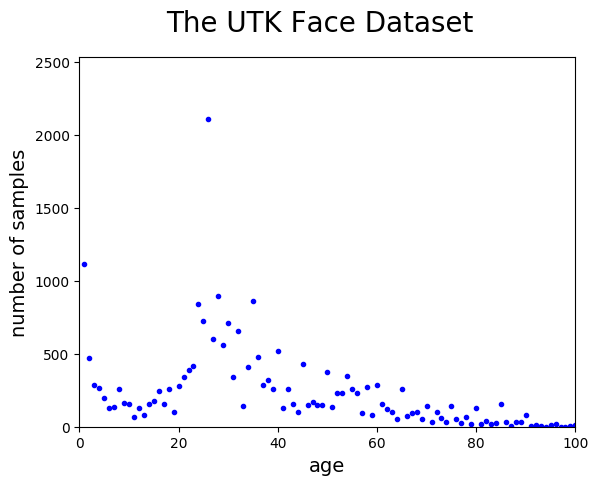
\includegraphics[width=13cm]{utk-stats}
\caption{Number of samples per age in the UTK Face Dataset}
\label{fig:utk-stats}
\end{figure}

\begin{figure}[h]
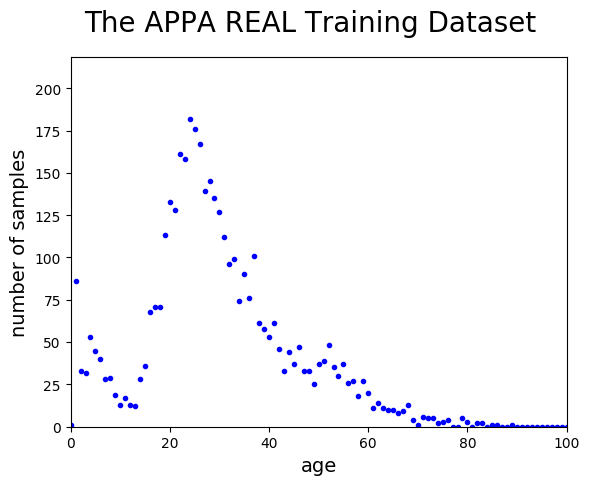
\includegraphics[width=13cm]{appa-train}
\caption{Number of samples per age in the APPA-REAL Training Dataset}
\label{fig:appa-train-stats}
\end{figure}

Instead of training a DNN from scratch, I used a pretrained DNN that is trained on the ImageNet dataset and fine-tuned it for age estimation. In other words, I downloaded already existing model of a DNN and re-trained it for my specific task, i.e. age estimation. This technique is called \textit{transfer learning} and more information about it can be found in \cite{yosinski2014transferable}.

If a person who is 65 years old gets classified as 66 years old, a classifier did actually a good job although it didn't predict the correct class. However, if a person who is 65 years old gets classified as 6 years old, that is a significantly bigger mistake than classifying it as 66 years old. Yet, when computing an accuracy, there is no difference if a predicted class is 6 or 66 if a ground truth is 65. That is the reason why in age estimation usually a mean absolute error (MAE) of a classifier is measured instead of accuracy.

When it comes to (targeted) misclassification, there is something in the age estimation domain that needs to be taken care of. If a person is classified a year or two older, it is not a huge success for a (targeted) misclassification. In the experiments that follow, targeted version of attacks is used, but a label is set as follows. If a person is under 50 years old, the target label is 90 years old. If a person is 50 years old or older, the target label is 10 years old. 

Formally, let $y$ be the ground truth label of an input sample $\pmb x$. Then function $f(y)$ is a function that outputs the target label for the corresponding sample $\pmb x$. The function $f$ is defined as

\begin{equation}
  f(y)=\left\{
  \begin{array}{@{}ll@{}}
       10, & \text{if } y \leq 50 \\
   	  90 & \text{otherwise }
  \end{array}\right.
\end{equation} 

The idea behind such a setting is to maximize the mean absolute error, i.e. make the classification as wrong as possible, using the targeted version of known attacks.  This is how I reused targeted attacks in a novel setting. Initially I put targeted labels to 0 and 100 instead of 10 and 90, respectively, but I observed a worse performance, probably because they are on the edge of the considered age range.

Two different optimizers are used in the experiments for minimizing a loss function: SGD, introduced in Section \ref{subsection:gradient-descent}, and Adam \cite{DBLP:journals/corr/KingmaB14}. Three different DNN architectures are used for training: VGG16 \cite{DBLP:journals/corr/SimonyanZ14a}, ResNet-50 \cite{DBLP:journals/corr/HeZRS15}, and InceptionResNetV2\cite{DBLP:journals/corr/SzegedyIV16}. Results of training the models based on the ResNet-50 architecture and the InceptionResNetV2 architecture are presented in Table \ref{table:trained-models}. 

The VGG16 architecture didn't show nearly as good results as the other two did, i.e. it always predicted the value of the most frequent label. Hence, I do not present the results of training the VGG16 in Table \ref{table:trained-models} and I do not evaluate any adversarial attack against it. However, if the VGG16 architecture is trained on the significantly larger IMDB-WIKI dataset, it can produce good results \cite{Rothe-IJCV-2016}. 

\begin{table}[]
\centering
\begin{tabular}{|c|c|c|c|c|}
\hline
Id & Architecture & Optimizer & Validation Loss & \textbf{Validation MAE} \\ \hline
1 & ResNet-50 & SGD & 3.436 & 5.151 \\ \hline
2 & ResNet-50 & Adam & 3.456 & 6.772 \\ \hline
3 & InceptionResNetV2 & SGD & 3.086 & 4.505  \\ \hline
4 & InceptionResNetV2 & Adam & 3.268 & 3.922 \\ \hline
\end{tabular}
\caption{Different models trained}
\label{table:trained-models}
\end{table}

For the evaluation of attacks, 100 random samples are taken from the APPA-REAL test dataset. Neither of the models from Table \ref{table:trained-models} has ever been trained on any of these samples before.


\section{Whitebox attacks}
\label{sec:whitebox-attacks}
When it comes to whitebox attacks, three approaches are evaluated: FGSM, CW and JSMA. Hyperparameters used in the FGSM and the CW attack are listed in Table \ref{table:fgsm-params} and Table \ref{table:cw-params}, respectively. In Table \ref{table:whitebox-results} results are presented.

It is interesting to notice that the FGSM attack managed to change MAE for the model with id 2 from 9.5 to 47.79. In other words, the targeted model on average predicted that a person in the adversarial image is 38 years younger or older than a person in the original image! 

Several original samples and the corresponding adversarial samples crafted in this experiment are presented in Figure \label{fig:fgsm-attack}. It can be observed that the attack adds a similar pattern to every image. However, when hyperparameter $eps$ is reduced to $1.0$, it is almost impossible to notice the perturbation as it can be seen in Figure \label{fig:fgsm-attack-eps1}. But it still can be noticed that there is some perturbation. Lines in adversarial images are not that sharp as in original images and some pixels are not natural e.g. line between left cheek and the background in the image (d).

\begin{figure}

\begin{subfigure}{.5\textwidth}
  \centering
  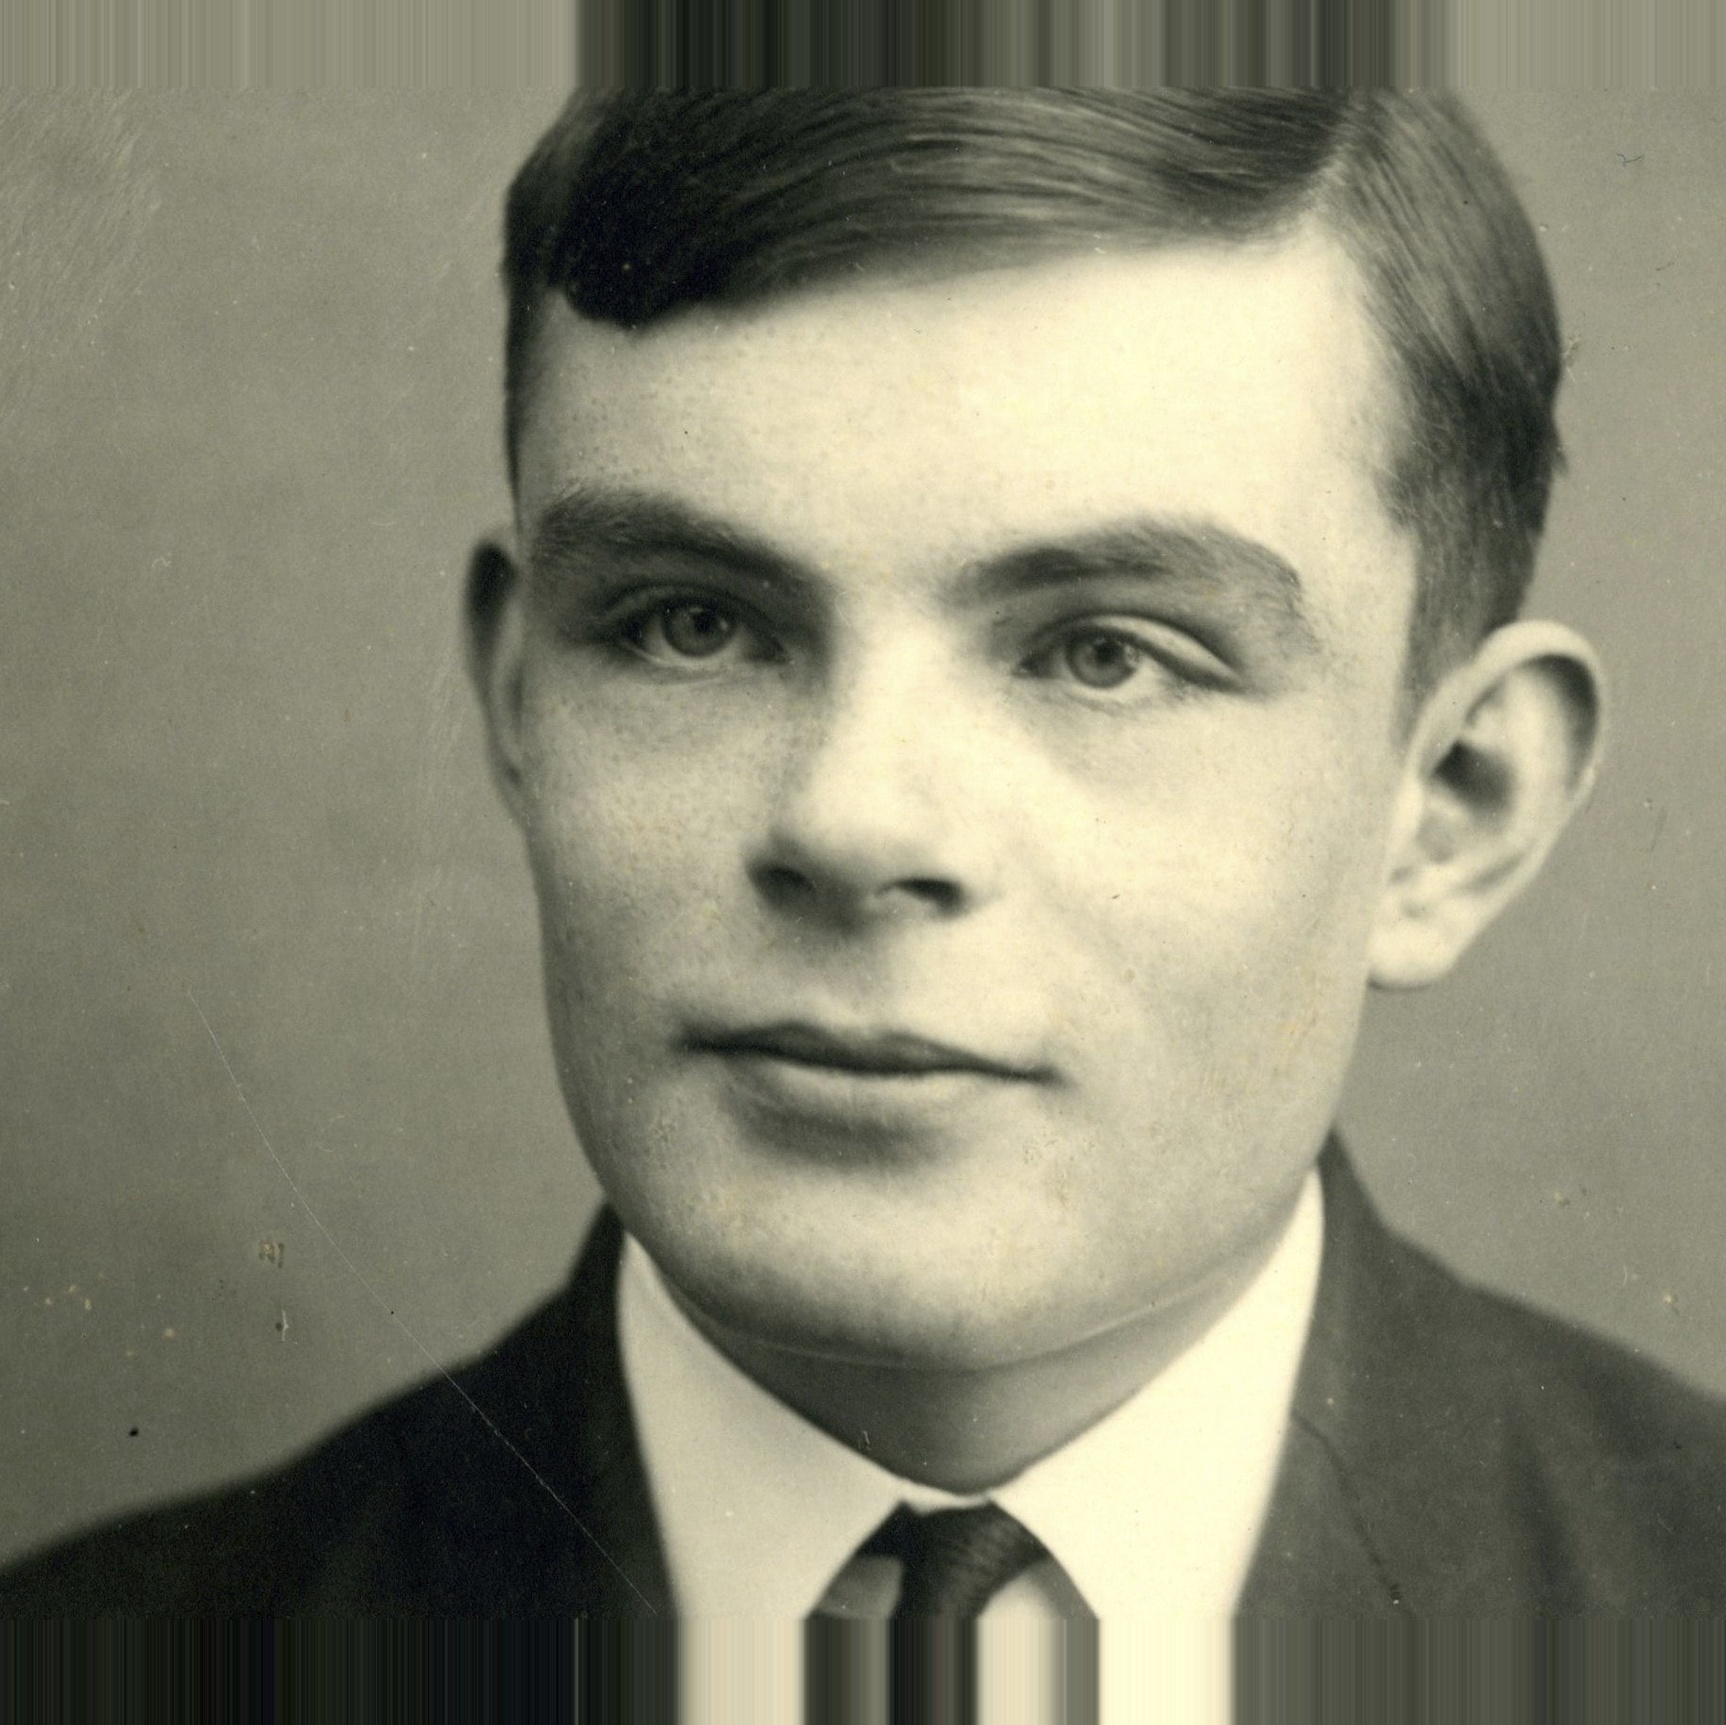
\includegraphics[height=5cm, width=\linewidth, keepaspectratio]{original_image_fgsm_1.jpg}
  \caption{Original sample classified as 28 years old}
\end{subfigure}
\begin{subfigure}{.5\textwidth}
  \centering
  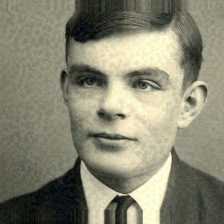
\includegraphics[height=5cm, width=\linewidth, keepaspectratio]{adversarial_image_fgsm_1.jpg}
  \caption{Adversarial sample classified as 85 years old}
\end{subfigure}

\begin{subfigure}{.5\textwidth}
  \centering
  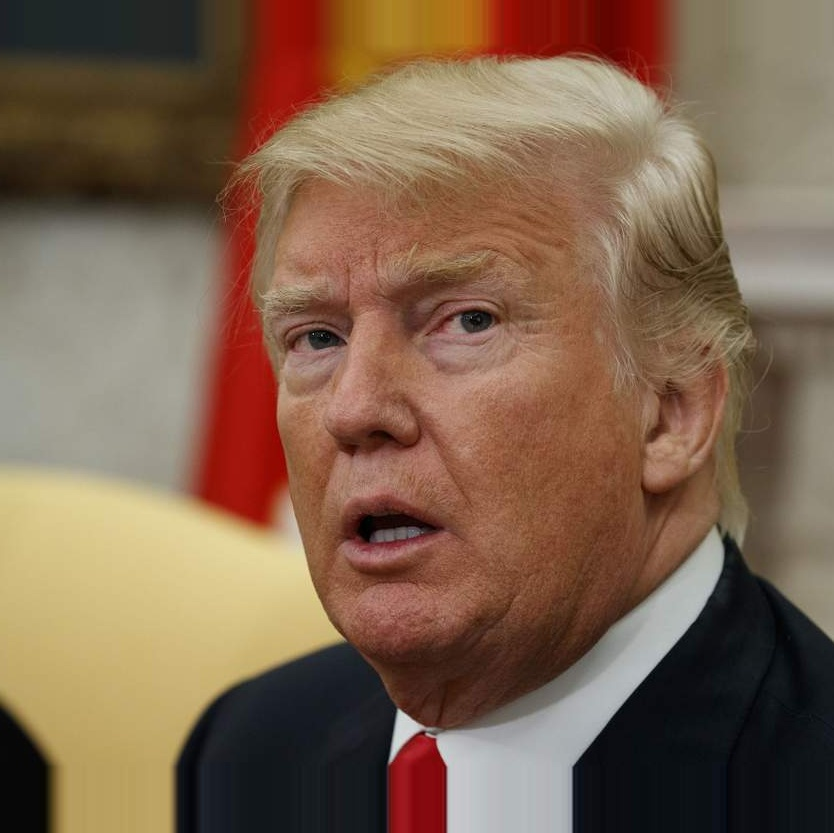
\includegraphics[height=5cm, width=\linewidth, keepaspectratio]{original_image_fgsm_2.jpg}
  \caption{Original sample classified as 59 years old}
\end{subfigure}
\begin{subfigure}{.5\textwidth}
  \centering
  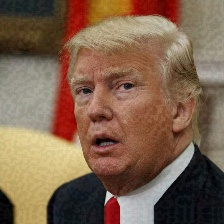
\includegraphics[height=5cm, width=\linewidth, keepaspectratio]{adversarial_image_fgsm_2.jpg}
  \caption{Adversarial sample classified as 23 years old}
\end{subfigure}

\begin{subfigure}{.5\textwidth}
  \centering
  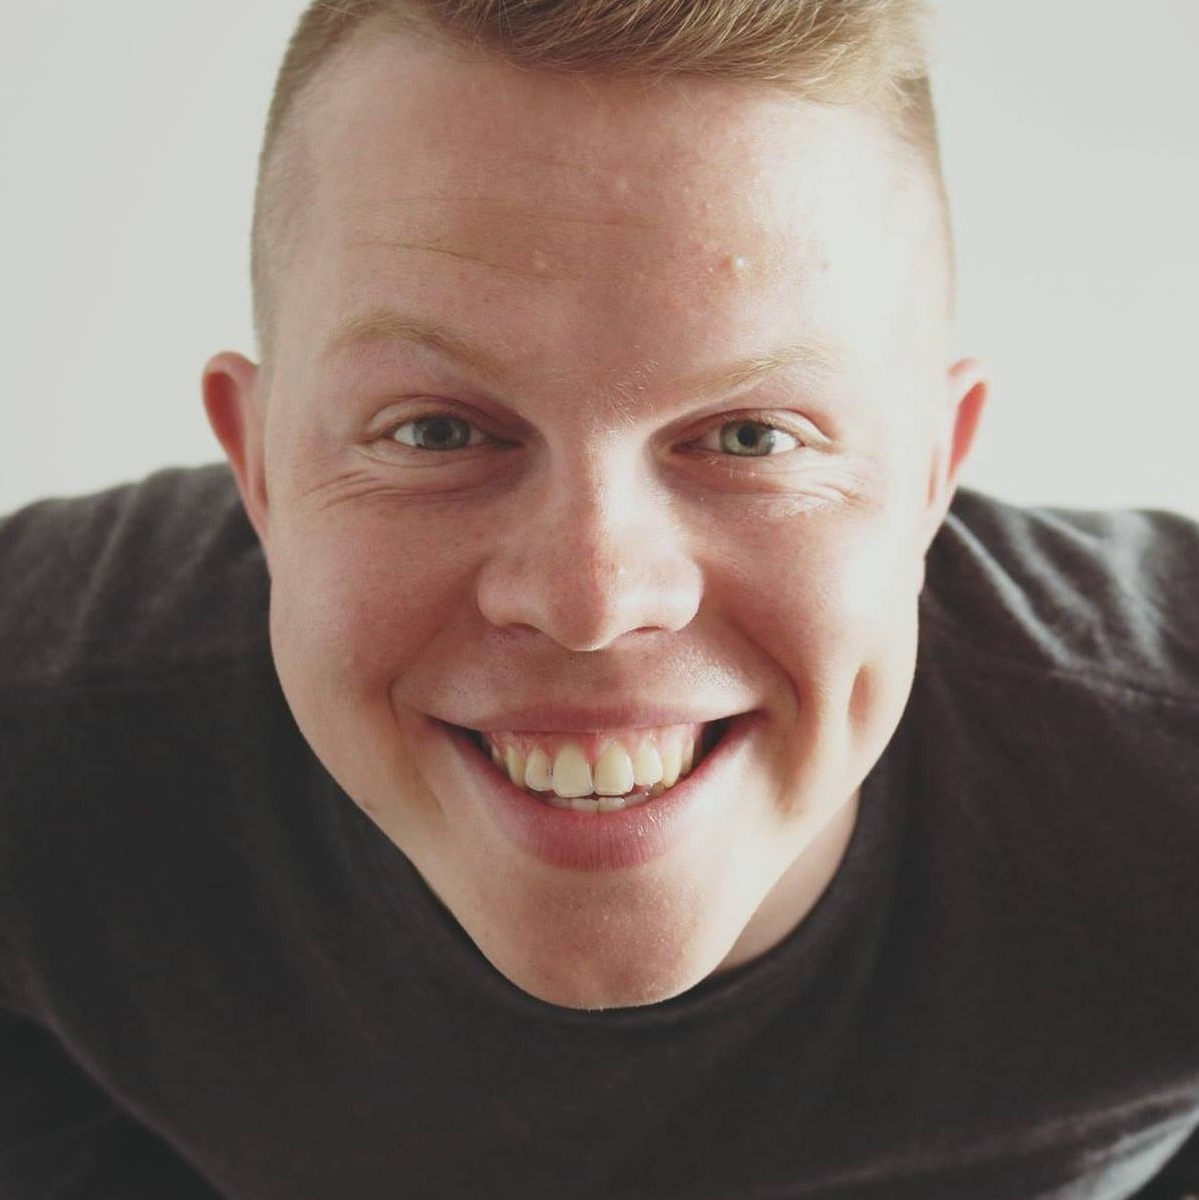
\includegraphics[height=5cm, width=\linewidth, keepaspectratio]{original_image_fgsm_3.jpg}
  \caption{Original sample classified as 28 years old}
\end{subfigure}
\begin{subfigure}{.5\textwidth}
  \centering
  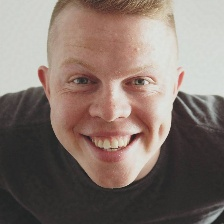
\includegraphics[height=5cm, width=\linewidth, keepaspectratio]{adversarial_image_fgsm_3.jpg}
  \caption{Adversarial sample classified as 85 years old}
\end{subfigure}

\caption{Original samples (left) and adversarial samples (right) crafted using the FGSM algorithm (\textit{eps} set to 5.0) and evaluated against the model with id 2}
\label{fig:fgsm-attack}
\end{figure}

\begin{figure}

\begin{subfigure}{.5\textwidth}
  \centering
  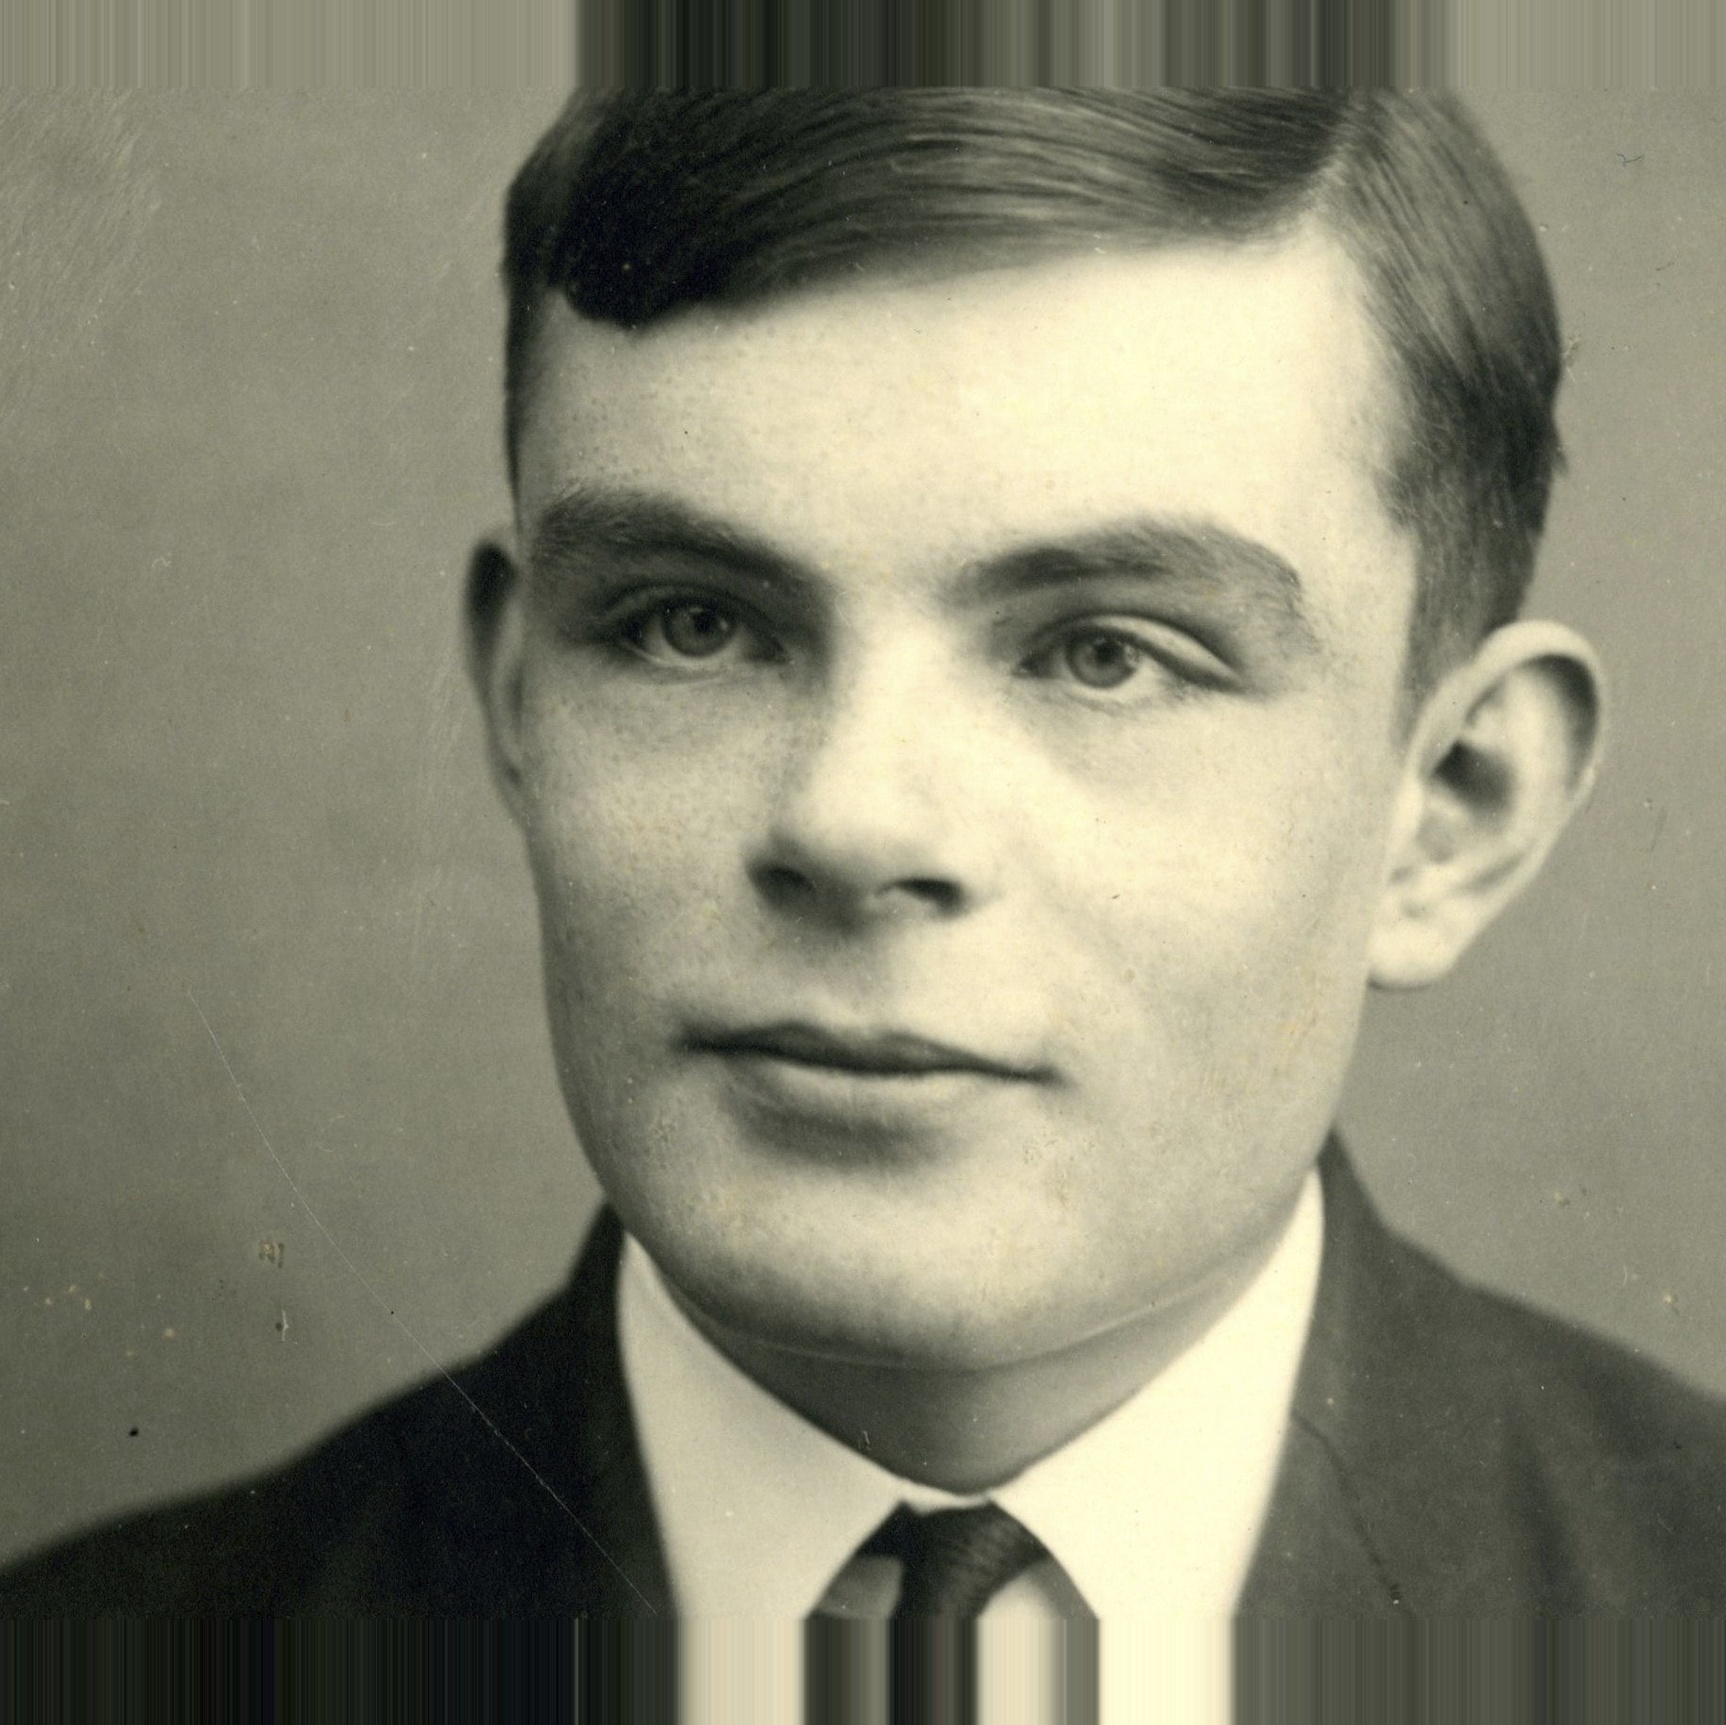
\includegraphics[height=5cm, width=\linewidth, keepaspectratio]{original_image_fgsm_1-eps1.jpg}
  \caption{Original sample classified as 28 years old}
\end{subfigure}
\begin{subfigure}{.5\textwidth}
  \centering
  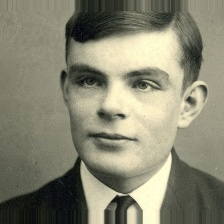
\includegraphics[height=5cm, width=\linewidth, keepaspectratio]{adversarial_image_fgsm_1-eps1.jpg}
  \caption{Adversarial sample classified as 59 years old}
\end{subfigure}

\begin{subfigure}{.5\textwidth}
  \centering
  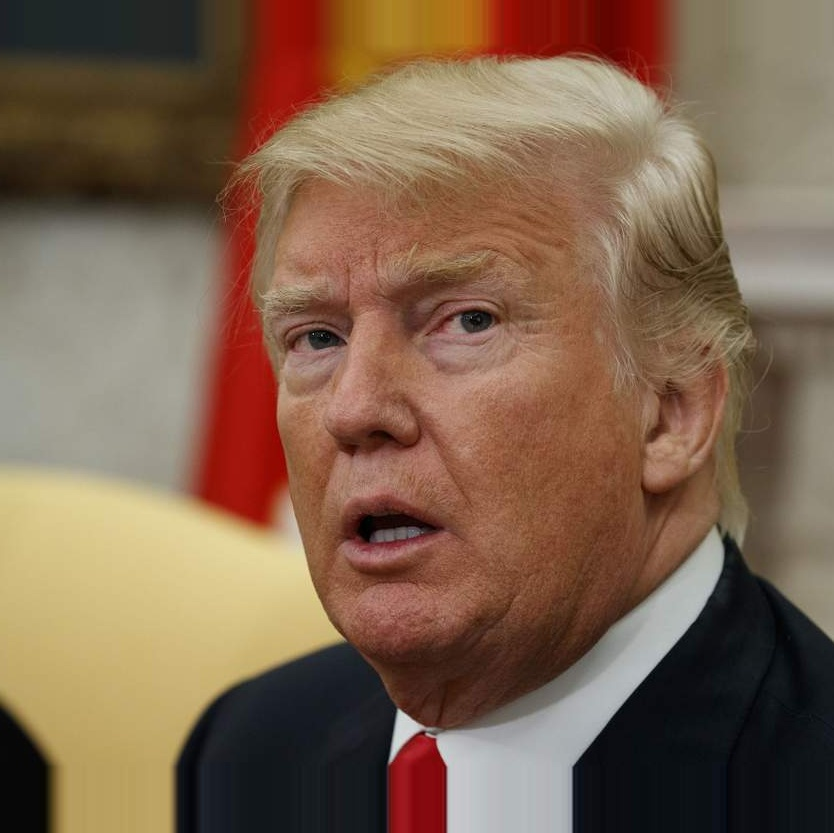
\includegraphics[height=5cm, width=\linewidth, keepaspectratio]{original_image_fgsm_2-eps1.jpg}
  \caption{Original sample classified as 59 years old}
\end{subfigure}
\begin{subfigure}{.5\textwidth}
  \centering
  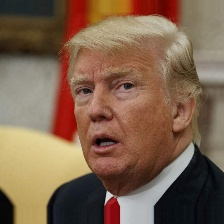
\includegraphics[height=5cm, width=\linewidth, keepaspectratio]{adversarial_image_fgsm_2-eps1.jpg}
  \caption{Adversarial sample classified as 28 years old}
\end{subfigure}

\begin{subfigure}{.5\textwidth}
  \centering
  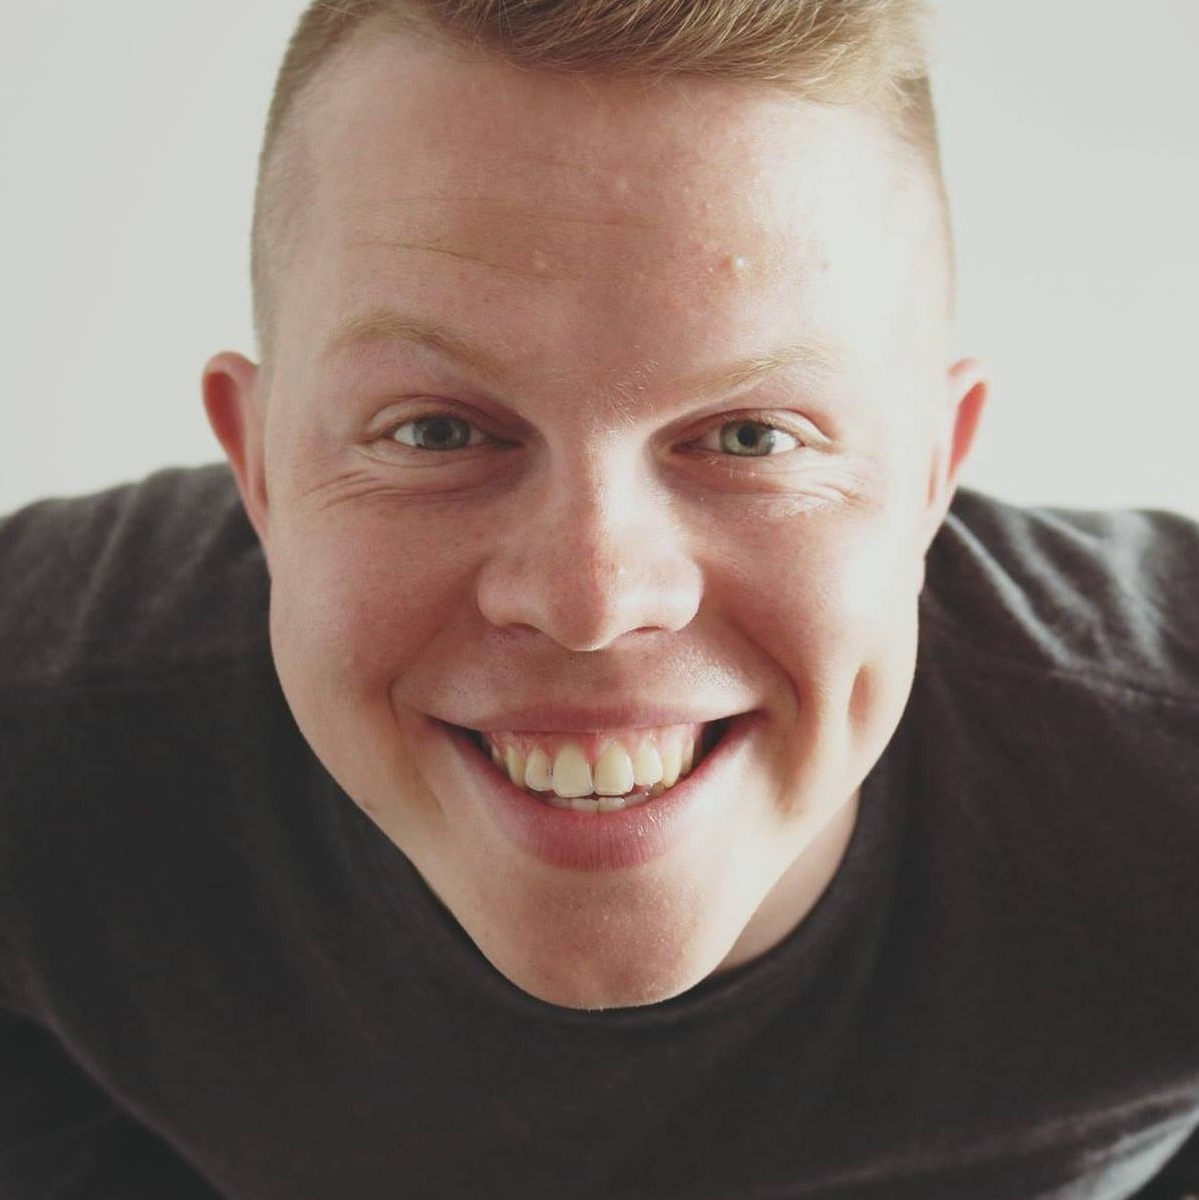
\includegraphics[height=5cm, width=\linewidth, keepaspectratio]{original_image_fgsm_3-eps1.jpg}
  \caption{Original sample classified as 28 years old}
\end{subfigure}
\begin{subfigure}{.5\textwidth}
  \centering
  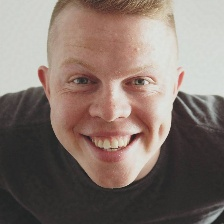
\includegraphics[height=5cm, width=\linewidth, keepaspectratio]{adversarial_image_fgsm_3-eps1.jpg}
  \caption{Adversarial sample classified as 64 years old}
\end{subfigure}

\caption{Original samples (left) and adversarial samples (right) crafted using the FGSM algorithm (\textit{eps} set to 1.0) and evaluated against the model with id 2}
\label{fig:fgsm-attack-eps1}
\end{figure}


The CW attack, given the hyperparameters in Table \ref{table:cw-params}, managed to move MAE for model with id 1 from 6.69 to 29.45.  In other words, the targeted model on average predicted that a person in the adversarial image is 23 years younger or older than a person in the original image. This is not that much as FGSM managed for the model with id 2, but it is significant.

TODO: Add sample image for CW

Since CW attack wasn't able to find any adversarial sample for the model with id 2 with the given hyperparameters in Table \ref{table:cw-params}, further experiments are performed against that model with different values for learning rate and maximum number of iterations.

Results of those experiments are presented in Table \ref{table:cw-results}. The results show that it is not easy for CW attack to find any adversarial sample on a specific model. Although no adversarial sample is found, I performed no further exploration of combination of learning rate and number of iterations. Further argumentation of this decision can be found in Section \ref{sec:threats-to-validity}.

It is also interesting to notice that for models with id 1 and 2, the attacks find stronger adversarial samples (i.e. bigger change in MAE) than for models with id 3 and 4. Could it be that bigger models \footnote{ResNet50 architecture that is used for model 1 and 2 has 25,636,712 parameters and InceptionResNetV2  architecture that is used for model 3 and 4 has 55,873,736 parameters.} are more resistent to adversarial samples? 

As expected from the analysis of the paper \cite{DBLP:journals/corr/CarliniW16a} in Section \ref{sec:CW}, JSMA attack failed due to memory complexity of the algorithm.

\begin{table}[]
\centering
\begin{tabular}{|c|c|}
\hline
eps & 5 \\  \hline
clip min & 0  \\ \hline
clip max & 255 \\ \hline
y\_target & 10 or 90 \\ \hline
\end{tabular}
\caption{Values of the hyperparameters used in the FGSM attack}
\label{table:fgsm-params}
\end{table}

\begin{table}[]
\centering
\begin{tabular}{|c|c|}
\hline
binary\_search\_steps & 8 \\ \hline
y\_target & 10 or 90 \\ \hline
abort\_early & True \\ \hline
max\_iterations & 5000 \\ \hline
learning\_rate & 1 \\ \hline
clip\_max & 255 \\ \hline
clip\_min & 0 \\ \hline
initial\_const & 0.1 \\ \hline
\end{tabular}
\caption{Values of the hyperparameters  used in the CW attack}
\label{table:cw-params}
\end{table}

\begin{table}[]
\centering
\begin{tabular}{|cccccccc|}
\hline
\multicolumn{2}{|c|}{} & \multicolumn{2}{c|}{FGSM} & \multicolumn{2}{c|}{CW} & \multicolumn{2}{c|}{JSMA} \\ \hline
\multicolumn{1}{|c|}{\begin{tabular}[c]{@{}c@{}}model\\ id\end{tabular}} & \multicolumn{1}{c|}{\begin{tabular}[c]{@{}c@{}}clean\\ MAE\end{tabular}} & \multicolumn{1}{c|}{\begin{tabular}[c]{@{}c@{}}adv\\ MAE\end{tabular}} & \multicolumn{1}{c|}{\begin{tabular}[c]{@{}c@{}}avg\\ L2\end{tabular}} & \multicolumn{1}{c|}{\begin{tabular}[c]{@{}c@{}}adv\\ MAE\end{tabular}} & \multicolumn{1}{c|}{\begin{tabular}[c]{@{}c@{}}avg\\ L2\end{tabular}} & \multicolumn{1}{c|}{\begin{tabular}[c]{@{}c@{}}adv\\ MAE\end{tabular}} & \multicolumn{1}{c|}{\begin{tabular}[c]{@{}c@{}}avg\\ L2\end{tabular}} \\ \hline
1 & 6.69 & 32.25 & 1879.63 & 29.45 & 2952.22 & - & - \\ \hline
2 & 9.5 & 47.79 & 1879.49 & 9.5 & 0.0 & - & - \\ \hline
3 & 5.4 & 19.32 & 2510.92 & 6.39 & 1175.80 & - & - \\ \hline
4 & 4.62 & 15.03 & 2511.10 & 7.14 & 1084.08 & - & - \\ \hline
\end{tabular}
\caption{Results of different adversarial attacks. The "-" sign means that an attack couldn't be executed.}
\label{table:whitebox-results}
\end{table}

\begin{table}[]
\begin{tabular}{|c|c|c|c|c|}
\hline
max iterations & learning rate & clean MAE & adv MAE & avg L2 \\ \hline
5 000 & 1 & 9.5 & 9.5 & 0.0 \\ \hline
10 000 & 1 & 9.5 & TODO & TODO \\ \hline
10 000 & 0.1 & 9.5 & 9.5 & 0.0 \\ \hline
10 000 & 10.0 & 9.5 & 9.5 & 0.0 \\ \hline
100 000 & 0.01 & 9.5 & 9.5 & 0.0 \\ \hline
\end{tabular}
\caption{Results using the CW attack with different values of hyperparameters against model with id 2}
\label{table:cw-results}
\end{table}

\section{Blackbox attacks}
\label{sec:blackbox-attacks}
When it comes to blackbox attacks, three approaches are evaluated: Transfer based approach, Ensemble approach and Boundary attack.

In the transfer based approach, first the targeted blackbox is queried with 100 different images and MAE is computed. Then a substitute network is trained using those 100 images. However, labels for those images are obtained by querying the targeted blackbox. Then the dataset is iteratively expanded via jacobian dataset augmentation technique . Finally, the FGSM attack is used to produce adversarial samples. Results are presented in the table XY.

Regarding the ensemble approach, ???

Finally, when it comes to boundary attack, I start with the image of 50 years old and make it look as 10, 20, 30, 40, 60, 70, 80 and 90 years old. Every attack is limited to 10 000 queries. Results are presented in image XY and table XY.




\chapter{The Semi-targeted Approach}
\label{chap:semi-targeted}
In Section \ref{sec:blackbox-attacks} I present observation that the transfer based approach expects more memory than it is available to me. In the same section I also present poor results of transfer based approach without Jacobian Augmentation. In this chapter I introduce an adaptation of the transfer based approach.

\section{Motivation}
High memory expectation, poor results without jacobian augmentation, and higher transferability of adversarial samples crafted in misclassification attacks than transferability of adversarial samples crafted in targeted misclassification attacks \cite{ensemble-attack} motivated me to modify transfer based approach.

In the modified approach the substitute network has lower number of classes than black-box model is expected to have and the goal of an attack against the substitute network is not targeted misclassification, but only misclassification. I call the modified approach \textit{the semi-targeted approach}.

In the semi targeted approach a substitute neural network has only a several classes and every class represents a certain age interval. If a misclassification occurs in such a scenario, that means that the classifier is tricked at least for the amount of years corresponding to the age interval. In this thesis all age intervals have the same length, but in general this is not necessary.

Let me provide an example. Assume a substitute network with only three classes that represent age intervals 0-33, 34-66 and 67-99 years. Now if a person who is 50 years old gets misclassified, that means the person got classified as 0-33 years old or as 67-99 years old. In either case, the mistake is greater than getting classified as 51 or 49 years old as it would be the case when the substitute network would have 100 classes. Finally, if that adversarial sample transfers to targeted black-box network, then the black-box model will also have a large error.

\section{Evaluation}
To make the semi-targeted approach and the transfer based approach comparable, hyperparameters of the FGSM and CW attacks as well as training and test samples are completely the same as in Section \ref{sec:blackbox-attacks}. Jacobian Augmentation is performed for several iterations before executing an attack as described in Section \ref{sec:transfer-based} that describes the transfer based approach .

However, in this approach the substitute network has fewer classes than the targeted black-box network. In performed experiments, the substitute network recognizes only three classes: 0-33, 34-66 and 67-99 years. Number of iterations for Jacobian Augmentation is 3. I also tried with 4 iterations for Jacobian Augmentation, but the system crashed. Number of epochs used for training the substitute network is set to 40.

Since the substitute network is trained on three classes, accuracy is used as a measure for evaluation of the network. For the targeted black-box neural network, MAE is used as a measure.



%\chapter{Critical Reflection}
%\section{Discussion}
\label{sec:discussion}
\input{chapters/critical-reflection/sections/discussion.tex}

\section{Threats to validity}
\label{sec:threats-to-validity}
Skipping the Jacobian-based Dataset Augmentation step in transfer based approach.

One could argue that without the jacobian augmentation, the transfer based approach is incomplete algorithm. Given the hardware resources \footnote{Intel(R) Core(TM) i5-8500 2 CPU @ 3.00GHz, 16GB RAM, GeForce GTX 1080 8GB}, every time during the call for jacobian augmentation, process would get killed by the kernel due to memory consumption. The implementation of the jacobian augmentation that is used is the offical one provided by the author \cite{papernot2018cleverhans}. I tried to contact the author \footnote{https://github.com/tensorflow/cleverhans/issues/974}, but even he couldn't find a solution \footnote{https://stackoverflow.com/questions/54580105/memory-consumption-of-jacobian-dataset-augmentation/54718059}. However, I observed that when the number of potential classes is lower, the jacobian-based augmentation can be performed for the same network.



\chapter{Threats to Validity and Future Work}
\label{chap:threats}
TODO: Discuss potential consequences of the decisions made

\section{Threats to Validity}
\label{sec:threats-to-validity}
\begin{itemize}

	\item \textbf{Decision:} Skipping the Jacobian-based Dataset Augmentation step in the transfer-based approach.

		\begin{itemize}	
			\item \textbf{Argumentation:} One could argue that without the Jacobian augmentation, the transfer based approach is an incomplete algorithm. Given the hardware resources\footnote{Intel(R) Core(TM) i5-8500 2 CPU @ 3.00GHz, 16GB RAM, GeForce GTX 1080 8GB}, every time during the call for Jacobian augmentation, the process would get killed by the kernel due to memory consumption. The implementation of the Jacobian augmentation that is used is the offical one provided by the author \cite{papernot2018cleverhans}. I tried to contact the author \footnote{https://github.com/tensorflow/cleverhans/issues/974}, but even he couldn't find a solution \footnote{https://stackoverflow.com/questions/54580105/memory-consumption-of-jacobian-dataset-augmentation/54718059}. However, I observed that when the number of potential classes is lower, the jacobian-based augmentation can be performed for the same network.
	
			\item \textbf{Potential consequences:} Since the transfer-based approach is not evaluated using the hardware that would support a complete execution of the attack, the results differ from those reported when a complete execution of the attack is supported.
		\end{itemize}
	
	\item \textbf{Decision:} Number of iterations for Jacobian-based Dataset Augmentations is too low in semi-targeted approach.

		\begin{itemize}
			\item \textbf{Argumentation:} Using the given resources, that are described above, it was not possible to perform more iterations.
	
			\item \textbf{Potential consequences:} The results are probably not as good as they would be when more iterations would be executed.
		\end{itemize}
	
	\item \textbf{Decision:} 
Not trying more than 100 000 iterations for CW attack in the whitebox experiment discussed in Section \ref{sec:whitebox-attacks}.

		\begin{itemize}
			\item \textbf{Argumentation:} The attack using 100 000 iterations takes a week to finish given the hardware resources. I believe that the hardware resources used in this thesis are hardware resources that an average adversarial user might have at hand and I don't see a motivation to run the attack for one sample for more than one week.
	
			\item \textbf{Potential consequences:} Given more iterations, an optimizer might do a better job.
		\end{itemize}
\end{itemize}








\section{Future Work}
\label{sec:future-work}
Reducing the complexity of Jacobian-based dataset augmentation would allow more people to experiment in this field without the need for too expensive resources. If the complexity can not be reduced, maybe another, memory efficient, heuristic can be used for obtaining boundaries of the targeted network. Eventually, this would allow attacks from cheap computers and raise the awareness about the security of neural networks.

If the resources allow, it would be interesting to evaluate the ensemble approach on this problem. A cluster can be constructed that would train different networks which would train based on the results of the black-box network. Then an adversarial sample for all of them would probably be adversarial against the black-box network as well.

It would be interesting to evaluate the black-box attacks presented in this thesis against the real world systems for age estimation that are publicly available. Microsoft Azure \footnote{https://azure.microsoft.com} is one such system which offers age estimation service. Before the evaluation against the real system, the experiments for black-box attacks should show better results.



\chapter{Summary}
\label{chap:summary}
TODO

\backmatter

% Use an optional list of figures.
%\listoffigures % Starred version, i.e., \listoffigures*, removes the toc entry.

% Use an optional list of tables.
%\cleardoublepage % Start list of tables on the next empty right hand page.
%\listoftables % Starred version, i.e., \listoftables*, removes the toc entry.

% Use an optional list of alogrithms.
%\listofalgorithms
%\addcontentsline{toc}{chapter}{List of Algorithms}

% Add an index.
\printindex

% Add a glossary.
\printglossaries

% Add a bibliography.
\bibliographystyle{alpha}
\bibliography{thesis-bibliography}

\end{document}
